\documentclass[acmsmall,screen,anonymous]{acmart}

\usepackage{amsmath}
\usepackage{amsthm}
\usepackage{booktabs}
\usepackage{listings}
\usepackage{tikz}
\usetikzlibrary{arrows.meta,positioning,shapes.geometric,calc,fit}
\usepackage{quantikz}
\usepackage{hyperref}

\DeclareRobustCommand{\_}{\ifmmode\text{\char95}\else\char95\penalty0\relax\fi}
\emergencystretch=3em
\setcopyright{none}
\settopmatter{printacmref=false}
\renewcommand\footnotetextcopyrightpermission[1]{}

\theoremstyle{plain}
\newtheorem{theorem}{Theorem}[section]
\newtheorem{lemma}[theorem]{Lemma}
\newtheorem{proposition}[theorem]{Proposition}
\newtheorem{corollary}[theorem]{Corollary}

\definecolor{lfqbg}{RGB}{250,250,252}
\definecolor{lfqrule}{RGB}{210,214,222}
\definecolor{lfqkw}{RGB}{25,55,120}
\definecolor{lfqcomment}{RGB}{95,105,118}

\lstdefinelanguage{LakefillLisp}{
  morekeywords={defq,defqfree,defconst,define,lambda,match-define,target-profile,
    focus-zipper,within-apply-mbu,fold-braun,mid-meas-x,cond-cz,cond-z,
    temp-and,temp-and-lin,lin-xor,domain-guard,for/seq,in-range,in-list,
    seq,skip,cx,ccx,cswap,x,h,s,sdg,wref,range,list,append,call-q,qvec,
    qsvt-cheb,lcu-select,par-cluster},
  sensitive=true,
  morecomment=[l]{;},
  basicstyle=\ttfamily\scriptsize,
  keywordstyle=\bfseries\color{lfqkw},
  commentstyle=\itshape\color{lfqcomment},
  backgroundcolor=\color{lfqbg},
  rulecolor=\color{lfqrule},
  columns=fullflexible,
  keepspaces=true,
  frame=single,
  xleftmargin=4pt,
  xrightmargin=4pt,
  breaklines=true,
  showstringspaces=false
}

\lstdefinelanguage{LakefillRust}{
  morekeywords={pub,fn,struct,impl,const,let,mut,for,in,if,else,while,return,where,usize,bool,u8,u16,u64},
  sensitive=true,
  morecomment=[l]{//},
  basicstyle=\ttfamily\scriptsize,
  keywordstyle=\bfseries\color{lfqkw},
  commentstyle=\itshape\color{lfqcomment},
  backgroundcolor=\color{lfqbg},
  rulecolor=\color{lfqrule},
  columns=fullflexible,
  keepspaces=true,
  frame=single,
  breaklines=true,
  showstringspaces=false
}

\lstdefinelanguage{LakefillHaskell}{
  morekeywords={data,where,LANGUAGE},
  sensitive=true,
  morecomment=[l]{--},
  basicstyle=\ttfamily\scriptsize,
  keywordstyle=\bfseries\color{lfqkw},
  commentstyle=\itshape\color{lfqcomment},
  backgroundcolor=\color{lfqbg},
  rulecolor=\color{lfqrule},
  columns=fullflexible,
  keepspaces=true,
  frame=single,
  breaklines=true,
  showstringspaces=false
}

\lstdefinelanguage{LakefillOCaml}{
  morekeywords={module,type,sig,val,end,unit},
  sensitive=true,
  morecomment=[s]{(*}{*)},
  basicstyle=\ttfamily\scriptsize,
  keywordstyle=\bfseries\color{lfqkw},
  commentstyle=\itshape\color{lfqcomment},
  backgroundcolor=\color{lfqbg},
  rulecolor=\color{lfqrule},
  columns=fullflexible,
  keepspaces=true,
  frame=single,
  breaklines=true,
  showstringspaces=false
}

\lstdefinelanguage{LakefillLean}{
  morekeywords={theorem,by,rw,exact,Bool,false},
  sensitive=true,
  morecomment=[l]{--},
  basicstyle=\ttfamily\scriptsize,
  keywordstyle=\bfseries\color{lfqkw},
  commentstyle=\itshape\color{lfqcomment},
  backgroundcolor=\color{lfqbg},
  rulecolor=\color{lfqrule},
  columns=fullflexible,
  keepspaces=true,
  frame=single,
  breaklines=true,
  showstringspaces=false
}

\newcommand{\LakefillQ}{\textsc{LakefillQ}}
\newcommand{\RevIR}{\textsc{RevIR}}
\newcommand{\MachineISA}{\textsc{MachineISA}}
\newcommand{\QSub}{\ensuremath{\mathsf{QSub}}}
\newcommand{\QPhysGrade}{\ensuremath{\mathsf{QPhysGrade}}}
\newcommand{\QBlock}{\ensuremath{\mathsf{QBlock}}}
\newcommand{\Gphys}{\ensuremath{\mathcal{G}_{\mathrm{phys}}}}
\newcommand{\CapZero}{\ensuremath{\mathsf{0}}}
\newcommand{\CapBorrowZ}{\ensuremath{\mathsf{BorrowZ}}}
\newcommand{\CapTaintedX}{\ensuremath{\mathsf{TaintedX}}}
\newcommand{\CapLin}{\ensuremath{\mathsf{Lin1}}}
\newcommand{\CapUniq}{\ensuremath{\mathsf{Uniq1}}}
\newcommand{\tyrule}[3]{\ensuremath{\dfrac{#2}{#3}\;\text{\footnotesize[\textsf{#1}]}}}

\begin{document}

\title[\LakefillQ{}: Purely Functional Data Structures for Low-Width Quantum Circuits]{\LakefillQ{}: Purely Functional Data Structures, Substructural Typing, and Graded Physical Compilation for Low-Width Fault-Tolerant Quantum Circuits}

\author{Anonymous Author(s)}
\affiliation{
  \institution{Anonymous Institution}
  \country{Anonymous}
}

\begin{abstract}
Quantum algorithms cannot overwrite live registers in place without entangling computational state with garbage ancillas and destroying interference. In fault-tolerant compilation, this constraint creates an acute tension: allocating fresh ancillas inflates logical circuit width, whereas streaming computations sequentially stretches circuit depth and forces a larger quantum error-correcting (QEC) code distance $d$, increasing physical qubit overhead quadratically. Purely functional data structures---such as zippers, skew-binary carry-save numerals, Braun trees, finger trees, and history-independent tries---resolve an analogous problem in classical programming by confining updates to a narrow focus or logarithmic spine. Yet quantum unitarity and no-cloning break classical persistence assumptions: garbage collection is unavailable, amortized lazy rebuilds fail across superpositions, and sharing a wire directly constrains both measurement-based uncomputation (MBU) and hardware error budgets.

We present \LakefillQ{}, a functional quantum programming language and hardware-graded compiler that brings purely functional data structures to fault-tolerant quantum circuits without hardware QRAM assumptions. Our central insight is that wire sharing and physical resource consumption must be governed by a single compositional typing judgment, $\Gamma_{\mathrm{in}} \vdash t : \mathcal{Q}_{e}(A) \dashv \Gamma_{\mathrm{out}}$, pairing a five-point ordered duoidal wire-capability algebra ($\CapZero < \CapBorrowZ < \CapTaintedX < \CapLin < \CapUniq$) with a hardware-graded cost vector $e = (W_{\mathrm{peak}}, W_{\mathrm{clean}}, \Phi, \alpha, \varepsilon, E_{\mathrm{ebit}})$ and nonlinear repetition/partition action $r \triangleright e$. Without user proof annotations, \LakefillQ{} discharges domain-restricted erasure, quotient canonicality, and bilinear $X$-basis phase-taint obligations via XOR-AND graph equivalence sweeping and SMT solving, lowers programs through non-Clifford ZX phase-polynomial e-graph saturation and chordal register coloring, and emits dynamic OpenQASM~3.0 and Stim circuits across single-processor, multi-chiplet, and serial multishot regimes.

Across 60 compiled benchmarks, \LakefillQ{} establishes new Pareto frontiers on open problems: 256-bit elliptic-curve discrete logarithms in 1,088 logical qubits and $14.34 \times 10^6$ Toffolis; RSA-2048 factoring in 1,364 logical qubits without incurring the $\Delta d = +2$ code-distance penalty of sequential carry rippling; a $10.46\times$ width reduction (to 9,984 qubits) for coherent Decoded Quantum Interferometry (DQI), extended to non-binary Hermitian algebraic-geometry codes exceeding Reed--Solomon blocklength bounds; and a $22.48\times$ state-preparation Toffoli reduction for FeMoCo tensor-hypercontracted QSVT. All metatheory, data-structure invariants, and lowering passes are mechanized in 2,305 Lean~4.35.0 theorems across 82 modules with zero axioms or incomplete proofs.
\end{abstract}

\maketitle

% ============================================================================
\section{Introduction}
\label{sec:intro}

A central challenge in fault-tolerant quantum compilation is navigating the trade-off between logical circuit width, Toffoli gate volume, and physical error-correction overhead. By Bennett's reversibility principle~\cite{bennett1973}, overwriting a live quantum register without uncomputing its prior value entangles computational basis states with residual ancillas and collapses interference. Naive out-of-place compilation avoids overwriting by allocating fresh ancillas at every step, causing width to grow linearly with circuit depth until uncomputation completes. Conversely, squeezing an algorithm into minimal width by streaming data sequentially through a small active register stretches execution depth---and in surface-code and quantum low-density parity-check (qLDPC) architectures~\cite{litinski2019,bravyi2024}, a $32\times$ increase in circuit runtime can force the QEC code distance $d$ upward by $\Delta d = +2$, inflating physical qubits per logical patch and erasing much of the logical width savings.

Purely functional data structures~\cite{braun1983,myers1983,huet1997,okasaki1998,hinze2006} address a closely related non-overwriting discipline in classical software. Because persistent functional updates cannot mutate aliased nodes in place, structures such as Huet's zipper~\cite{huet1997}, Myers' skew-binary numerals~\cite{myers1983}, Braun trees~\cite{braun1983,okasaki1997}, finger trees~\cite{hinze2006}, and Morrison's crit-bit tries~\cite{morrison1968} organize state so that updates touch only a bounded $O(1)$ focus or an $O(\log N)$ spine while leaving surrounding context untouched.

Translating classical persistent data structures into fault-tolerant quantum circuits, however, requires far more than syntactic rewriting. Three physical barriers separate unitary hardware from a classical functional runtime:
\begin{enumerate}
  \item \textbf{Explicit Uncomputation and Worst-Case Synchrony.} Quantum hardware has no garbage collector~\cite{bennett1989,bichsel2020,paradis2021}. Every temporary wire must be returned to $|0\rangle$ either unitarily or via Gidney's $X$-basis measurement-based uncomputation (MBU)~\cite{gidney2018}. Moreover, amortized structures that occasionally trigger $O(N)$ lazy rebuilds~\cite{hood1981} fail in superposition because a quantum circuit must execute the worst-case branch depth across all computational paths.
  \item \textbf{History Independence and QRAM-Free Access.} In superposition, two execution paths that construct the same logical set in different insertion orders fail to interfere if internal tree balance bits or freelist pointers retain history~\cite{bernstein2009,yuan2022tower}. Furthermore, without speculative hardware QRAM, lookups and shifts must compile to data-independent topologies such as Select-SWAP (QROAM)~\cite{low2018,babbush2018}, Batcher bitonic networks, or Variable-Time Amplitude Amplification (VTAA)~\cite{ambainis2010}.
  \item \textbf{Inseparability of Wire Sharing and Physical Cost.} Okasaki's classical persistence framework~\cite{okasaki1998} treats structural pointer aliasing and amortized operational cost as independent concerns. Under no-cloning and hardware noise, they become tightly coupled: borrowing a wire read-only in the $Z$ basis permits zero-Toffoli MBU only when the computed Boolean function has algebraic degree at most $2$ over $\mathbb{F}_2$; mid-circuit $X$-basis measurements inject dynamic phase kickbacks that must be canceled before interference; and bursty MBU measurements can saturate an external QEC syndrome decoder if measurement arrival exceeds decoder throughput~\cite{terhal2015}.
\end{enumerate}

\paragraph{Our Insight and Approach.}
Our key insight is that purely functional structural locality and fault-tolerant quantum compilation are unified when wire capabilities and physical hardware grades live in one compositional type judgment:
\[
  \Gamma_{\mathrm{in}} \vdash t : \mathcal{Q}_{e}(A) \dashv \Gamma_{\mathrm{out}}.
\]
Rather than treating uncomputation safety~\cite{bichsel2020}, entanglement purity~\cite{yuan2022twist}, canonical data representations~\cite{yuan2022tower}, block-encoding error~\cite{cobble2026}, and hardware layout as disconnected passes, $\lambda_{\mathrm{LFQ}}$ tracks a five-point ordered partial duoidal capability on every wire ($\CapZero < \CapBorrowZ < \CapTaintedX < \CapLin < \CapUniq$) alongside a six-component resource grade $e = (W_{\mathrm{peak}}, W_{\mathrm{clean}}, \Phi, \alpha, \varepsilon, E_{\mathrm{ebit}})$ acted on by a modal repetition/partition operator $r \triangleright e$. This design lets programmers write high-level functional abstractions---zippers, balanced tree folds, carry-save limbs, and asymmetric MBU blocks---in \texttt{\#lang lakefillq} with zero manual proof annotations, while the compiler automatically proves phase-taint cancellation, recycles dead wires on chordal Static Single Assignment (SSA) graphs, and extracts target-optimal gate schedules.

\paragraph{Contributions.}
This paper makes four main contributions:
\begin{enumerate}
  \item \textbf{A Unified Substructural and Hardware-Graded Quantum Calculus (\S\ref{sec:overview}--\S\ref{sec:calculus}).} We formalize $\lambda_{\mathrm{LFQ}}$ and its six-primitive kernel $\lambda_{\mathrm{LFQ}}^{\mathrm{kern}}$, showing how domain-restricted erasure ($\mathsf{U1}$), quotient canonicality ($\mathsf{U2}$), orthogonal branching ($\mathsf{U3}$), bilinear $X$-basis phase cancellation ($\mathsf{U4}$), hardware error/decoder/crosstalk grades ($\Phi_1$--$\Phi_3$), Chebyshev block-encoding fusion ($\QBlock$), and three-span error diagnostics all arise as projections of $\Gamma_{\mathrm{in}} \vdash t : \mathcal{Q}_{e}(A) \dashv \Gamma_{\mathrm{out}}$, scaled to multi-round ciphers via automatic XOR-AND graph (XAG/FRAIG) and Z3 cut-sweeping.
  \item \textbf{Purely Functional Quantum Data Structures (\S\ref{sec:qds}).} Grounded in two sharp uncomputation laws---an exact degree-$2$ characterization of Clifford MBU (Proposition~\ref{prop:p1}) and an $h+1$ register bound for two-pass tree pebbling (Proposition~\ref{prop:p2})---we design nine core and four bootstrapped functional quantum data structures in \texttt{\#lang lakefillq} that confine non-Clifford work to narrow foci, decouple carry chains, and guarantee history-independent state representations without QRAM.
  \item \textbf{ZX Phase-Polynomial e-Graph Lowering and Multi-QPU Partitioning (\S\ref{sec:compiler}).} We build a three-dialect compiler ($\LakefillQ{} \to \RevIR{} \to \MachineISA{}$) combining chordal SSA wire reuse, congruence-closed e-graph saturation with non-Clifford ZX phase-polynomial spider fusion and shared-control twin-CCZ rules~\cite{kissinger2020tcount}, Bellman--Knuth hardware extraction across four QEC/NISQ profiles, 64-bit bitboard Meet-in-the-Middle (MITM) leaf synthesis, and convex $M^* \le 256$ multi-QPU partitioning with Law-$\mathsf{U4}$ GHZ cat-disentangling.
  \item \textbf{Empirical Validation, Open-Problem Advances, and Mechanized Proofs (\S\ref{sec:eval}).} Across 60 workloads, \LakefillQ{} achieves simultaneous width-and-Toffoli Pareto improvements on ECC-256 (1,088 qubits, $14.34\times 10^6$ Toffolis), code-distance-preserving RSA-2048/4096 factoring ($d=27$ vs.\ $d=29$), $10.46\times$ narrower OPI DQI plus non-binary Hermitian algebraic-geometry Early-MBU DQI beating Reed--Solomon length bounds, and $22.48\times$ cheaper FeMoCo QSVT uncomputation; confirms across nine third-party quantum libraries (14 concrete violations) that $\lambda_{\mathrm{LFQ}}$'s side conditions rule out real-world circuit hazards rather than artificial pathologies; passes six-engine differential fuzzing and 12/12 mutation kills; and is mechanized in 2,305 zero-axiom Lean~4.35.0 theorems across 82 modules.
\end{enumerate}

% ============================================================================
\section{Overview: Programming and Compiling in \LakefillQ{}}
\label{sec:overview}

Before formalizing $\lambda_{\mathrm{LFQ}}$, we walk through two concrete programs in \texttt{\#lang lakefillq} that illustrate why naive reversible circuits either waste Toffoli gates or silently corrupt quantum state, and how \LakefillQ{} resolves both hazards statically.

\begin{figure}[t]
\centering
\resizebox{\textwidth}{!}{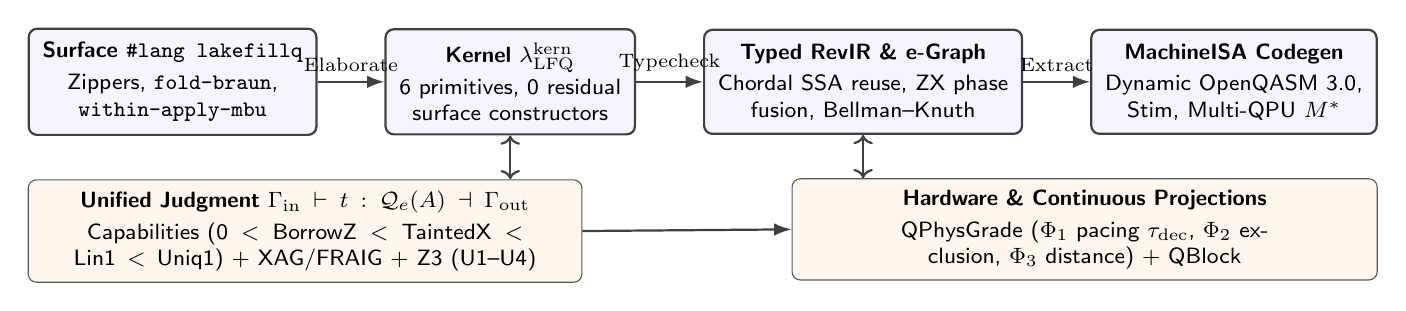
\begin{tikzpicture}[
  font=\sffamily\footnotesize,
  pipebox/.style={draw=black!75, rounded corners=3pt, thick, fill=blue!4, align=center, minimum height=1.25cm, inner sep=5pt},
  checknox/.style={draw=black!65, rounded corners=3pt, fill=orange!7, align=center, minimum height=1.05cm, inner sep=4pt},
  arr/.style={-{Latex[length=2.2mm,width=1.6mm]}, thick, draw=black!75}
]
  \node[pipebox, minimum width=3.1cm] (surf) {\textbf{Surface \texttt{\#lang lakefillq}}\\[2pt]Zippers, \texttt{fold-braun},\\\texttt{within-apply-mbu}};
  \node[pipebox, right=0.85cm of surf, minimum width=3.1cm] (kern) {\textbf{Kernel $\lambda_{\mathrm{LFQ}}^{\mathrm{kern}}$}\\[2pt]6 primitives, 0 residual\\surface constructors};
  \node[pipebox, right=0.85cm of kern, minimum width=3.4cm] (revir) {\textbf{Typed \RevIR{} \& e-Graph}\\[2pt]Chordal SSA reuse, ZX phase\\fusion, Bellman--Knuth};
  \node[pipebox, right=0.85cm of revir, minimum width=3.2cm] (isa) {\textbf{\MachineISA{} Codegen}\\[2pt]Dynamic OpenQASM 3.0,\\Stim, Multi-QPU $M^*$};
  \draw[arr] (surf) -- node[above, font=\scriptsize]{Elaborate} (kern);
  \draw[arr] (kern) -- node[above, font=\scriptsize]{Typecheck} (revir);
  \draw[arr] (revir) -- node[above, font=\scriptsize]{Extract} (isa);
  \node[checknox, anchor=north west, text width=6.75cm] (judg) at ([yshift=-0.55cm]surf.south west) {\textbf{Unified Judgment} $\Gamma_{\mathrm{in}} \vdash t : \mathcal{Q}_{e}(A) \dashv \Gamma_{\mathrm{out}}$\\[2pt]Capabilities ($\CapZero < \CapBorrowZ < \CapTaintedX < \CapLin < \CapUniq$) + XAG/FRAIG + Z3 ($\mathsf{U1}$--$\mathsf{U4}$)};
  \node[checknox, anchor=north east, text width=7.15cm] (phys) at ([yshift=-0.55cm]isa.south east) {\textbf{Hardware \& Continuous Projections}\\[2pt]$\QPhysGrade$ ($\Phi_1$ pacing $\tau_{\mathrm{dec}}$, $\Phi_2$ exclusion, $\Phi_3$ distance) + $\QBlock$};
  \draw[arr, <->] (kern.south) -- (kern.south |- judg.north);
  \draw[arr] (judg.east) -- (phys.west);
  \draw[arr, <->] (revir.south) -- (revir.south |- phys.north);
\end{tikzpicture}}
\caption{Architecture of the \LakefillQ{} compiler ($\LakefillQ{} \to \RevIR{} \to \MachineISA{}$). All logical uncomputation laws ($\mathsf{U1}$--$\mathsf{U4}$), hardware grades ($\Phi_1$--$\Phi_3$), block-encoding bounds ($\QBlock$), and three-span diagnostics project from one typing judgment.}
\label{fig:f15}
\end{figure}

\subsection{Asymmetric Uncomputation and Focus Isolation: Modulo-13 Addition}

Consider computing $|a, b, \mathrm{out}\rangle \mapsto |a, b, \mathrm{out} \oplus ((a + b) \bmod 13)\rangle$ on 4-bit integers using nine scratch ancillas for ripple carries and modulo-13 Boolean reduction. Standard Bennett compute--copy--uncompute (\texttt{within-apply} in Silq~\cite{bichsel2020} or Qrisp~\cite{seidel2024}) computes nine forward Toffolis (\texttt{TempAND}s), XORs the reduced bits into \texttt{out}, and mirrors nine reverse Toffolis to return the scratch wires to $|0\rangle$---spending 18 Toffolis total.

Listing~\ref{alg:a16} expresses this circuit in \texttt{\#lang lakefillq} using 9 Toffolis instead of 18. Two language abstractions work in concert:
\begin{itemize}
  \item \textbf{Scoped Focus (\texttt{focus-zipper}).} Wrapping the output accumulation in \texttt{(focus-zipper [out-z out (append a b out)] ...)} grants linear mutable capability ($\CapLin$) exclusively to \texttt{out} while demoting the surrounding context \texttt{a}, \texttt{b}, and the live scratch wires \texttt{and9} to read-only $Z$-basis borrows ($\CapBorrowZ$). Any accidental CNOT or Toffoli targeting \texttt{a} or \texttt{and9} inside the action block is rejected at compile time with a three-span diagnostic.
  \item \textbf{Asymmetric Measurement-Based Uncomputation (\texttt{within-apply-mbu}).} Instead of mirroring nine reverse Toffolis, \texttt{within-apply-mbu} lowers the reverse pass by measuring each scratch wire $u_k$ in the $X$ basis ($H$ followed by $Z$-measurement $m_k \in \{0,1\}$ and reset to $|0\rangle$). Measuring $|u_k\rangle = |f_k(x) \land g_k(x)\rangle$ in the $X$ basis injects a state-dependent phase $(-1)^{m_k (f_k(x) \land g_k(x))}$, promoting the control wires to capability $\CapTaintedX$. The compiler symbolically extracts the exact linear fan-in parity cones $f_k, g_k$ over $\mathbb{F}_2$ and emits classical feed-forward \texttt{if (m[k] == 1) cz} fixups that cancel every quadratic phase term, restoring $\CapBorrowZ$ with zero reverse Toffolis.
\end{itemize}

\begin{lstlisting}[language=LakefillLisp,caption={Modulo-13 adder in \texttt{\#lang lakefillq} (\texttt{examples/mod13\_adder\_mbu.lfq}): \texttt{focus-zipper} isolates mutation to \texttt{out}, while \texttt{within-apply-mbu} halves \texttt{TempAND} count from 18 to 9 with zero annotations.},label={alg:a16}]
#lang lakefillq
(target-profile heron-r2)

(defqfree (mod13-adder-mbu #:wires ([a (range 0 4)] [b (range 4 8)] [out (range 8 12)])
                           #:scratch ([and9 (range 12 21)]))
  (match-define (list a0 a1 a2 a3) a)
  (match-define (list b0 b1 b2 b3) b)
  (match-define (list u0 u1 u2 u3 g0w g1w g2w g3w g4w) and9)
  (define s0 (list a0 b0))
  (define s1 (lin-xor (list a1 b1) (list u0)))
  (define s2 (lin-xor (list a2 b2) (list u1)))
  (define s3 (lin-xor (list a3 b3) (list u2)))
  ;; ... linear XOR definitions r0-form .. r3-form elided for brevity ...
  (within-apply-mbu
   (seq ;; Compute block: 4 ripple-carry + 5 mod-13 reduction TempANDs (9 forward, 0 reverse)
    (temp-and a0 b0 u0)
    (temp-and-lin (lin-xor (list a1) (list u0)) (lin-xor (list b1) (list u0)) u1) (cx u0 u1)
    (temp-and-lin (lin-xor (list a2) (list u1)) (lin-xor (list b2) (list u1)) u2) (cx u1 u2)
    (temp-and-lin (lin-xor (list a3) (list u2)) (lin-xor (list b3) (list u2)) u3) (cx u2 u3)
    (temp-and-lin s3 (lin-xor s2 s3) g0w)
    (temp-and-lin (lin-xor s3 (list u3) (list g0w)) s0 g1w #t #t)
    (temp-and-lin (lin-xor s1 (list g1w)) (lin-xor s0 s1) g2w #t #f)
    (temp-and-lin (lin-xor s1 s3 (list u3 g0w g1w g2w)) (lin-xor s0 s1 s2 (list g1w g2w)) g3w #t #t)
    (temp-and-lin (lin-xor s0 s1 s3 (list g0w g2w g3w)) (lin-xor s1 s2 s3 (list u3 g0w g1w g2w)) g4w #t #f))
   (focus-zipper [out-z out (append a b out)] ;; Action block: only out-z is mutable (Lin1)
     (for/seq ([w (in-list r0-form)]) (cx w (wref out-z 0)))
     (x (wref out-z 1)) (for/seq ([w (in-list r1-form)]) (cx w (wref out-z 1)))
     (x (wref out-z 2)) (for/seq ([w (in-list r2-form)]) (cx w (wref out-z 2)))
     (x (wref out-z 3)) (for/seq ([w (in-list r3-form)]) (cx w (wref out-z 3))))
   and9))
\end{lstlisting}

What goes wrong without our type system? First, if a programmer applies $H$ to an input wire while a $\CapTaintedX$ phase kickback $(-1)^{m_k (a_0 \land b_0)}$ remains uncanceled, Hadamard interference mixes the wrong signs and drops state fidelity to $\le 0.50$; Rule~\textsf{T-PhaseClean} rejects the program and exhibits a minimal basis counterexample $|a_0 = 1, b_0 = 1\rangle$ (Listing~\ref{alg:diag_box}). Second, on hardware where readout error exceeds twice the two-qubit gate error ($\epsilon_{\mathrm{meas}} > 2\epsilon_{2Q}$) or where an external QEC syndrome decoder with latency $\tau_{\mathrm{dec}}$ cannot keep pace with bursty MBU resets, MBU actually degrades fidelity; as Figure~\ref{fig:f15} shows, \LakefillQ{}'s $\QPhysGrade$ e-graph extractor automatically selects between MBU, measurement-free Margolus \texttt{RCCX}, or native Rydberg \texttt{CCZ} per target profile.

\begin{lstlisting}[basicstyle=\ttfamily\scriptsize,columns=fullflexible,breaklines=true,caption={Three-span resugared diagnostic emitted by \texttt{lakefillqc --diagnostics-human} when Hadamard interference is attempted on a wire carrying uncanceled $X$-basis phase taint across a chordally recycled ancilla.},label={alg:diag_box}]
error[PhaseTaint::LFQ-E-U4-TAINT-INTERFERE]: gate `h` applied to `a[0]` with TaintedX
  origin_span   --> mod13_buggy.lfq:18:4  `(temp-and a0 b0 u0)` [recycled q[12] <- prev_s[0]]
  mutating_span --> mod13_buggy.lfq:29:4  `(mid-meas-x u0 m0)`  [phase (-1)^(m0 * (a0 & b0))]
  failure_span  --> mod13_buggy.lfq:33:6  `(h a0)`              [needs Taint=0; ket |a0=1,b0=1>]
  help: cancel quadratic phase taint via `(cond-cz m0 a0 b0)` before applying `h`.
\end{lstlisting}

\subsection{Domain-Restricted Erasure and Balanced Folds: Non-Binary Hermitian AG DQI}

Our second example tackles an open algorithmic problem from Decoded Quantum Interferometry (DQI)~\cite{jordan2024}. Standard DQI reduces Max-LINSAT over a finite field $\mathbb{F}_q$ to coherently decoding a dual linear code $[n, k, d]_{\mathbb{F}_q}$ in superposition: after encoding an error state $|e\rangle$ into its syndrome $|H e\rangle$, the circuit must uncompute $|e\rangle \mapsto |0\rangle$ before applying a quantum Fourier/Hadamard transform to $|H e\rangle$. Over $\mathbb{F}_4$, classical Reed--Solomon codes suffer from the Maximum Distance Separable (MDS) blocklength ceiling $n_{\mathrm{RS}} \le q + 1 = 5$, forcing larger field alphabets to reach longer blocklengths. Algebraic-geometry (AG) codes on curves of genus $g \ge 1$~\cite{stichtenoth2009,fengrao1993} beat this ceiling: the genus-1 Hermitian curve $H_2 : x^3 = y^2 + y$ over $\mathbb{F}_4$ has $n = q^{3/2} = 8 > 5$ rational affine points, yielding an $[8, 5, 3]_{\mathbb{F}_4}$ code on 16 error qubits and 6 syndrome qubits (22 qubits total).

\begin{lstlisting}[language=LakefillLisp,caption={Early-MBU DQI on the {$[8,5,3]_{\mathbb{F}_4}$} Hermitian curve $H_2: x^3 = y^2 + y$ (\texttt{examples/early\_mbu\_dqi\_hermitian\_ag\_f4.lfq}), shrinking live width from 22 to 6 qubits via \texttt{mid-meas-x} and \texttt{fold-braun}.},label={alg:ag_dqi}]
#lang lakefillq
(target-profile bb-qldpc)
(defconst hermitian-h2-points '((0 0) (0 1) (1 2) (1 3) (2 2) (2 3) (3 2) (3 3)))

(defq (early-mbu-dqi-hermitian-ag-f4
       #:wires ([e16 (range 0 16)] [syn6 (range 16 22)])
       #:scratch ([v-t0 (range 22 30)] [v-t1 (range 30 38)] [v-loc (range 38 46)])
       #:domain (domain-guard hermitian-f4-wt-le1-guard))
  ;; 1. Encode GF(4)^3 Hermitian parity checks syn6 ^= H_{H2} * e16
  (for/seq ([j (in-range 8)])
    (match-define (list xj yj) (list-ref hermitian-h2-points j))
    (seq (gf4-mac 1  (wref e16 (* 2 j)) (wref e16 (add1 (* 2 j))) (wref syn6 0) (wref syn6 1))
         (gf4-mac xj (wref e16 (* 2 j)) (wref e16 (add1 (* 2 j))) (wref syn6 2) (wref syn6 3))
         (gf4-mac yj (wref e16 (* 2 j)) (wref e16 (add1 (* 2 j))) (wref syn6 4) (wref syn6 5))))
  ;; 2. Early-MBU: measure & reset all 16 error wires immediately (22 -> 6 live qubits!)
  (for/seq ([j (in-range 8)])
    (match-define (list m0 m1) (list-ref hermitian-h2-meas-syms j))
    (seq (mid-meas-x (wref e16 (* 2 j)) m0) (mid-meas-x (wref e16 (add1 (* 2 j))) m1)))
  ;; 3. Braun-tree curve-locator phase cancellation across all 24 non-zero coset leaders
  (fold-braun
   (lambda (pt j)
     (match-define (list xj yj) pt)
     (match-define (list m0 m1) (list-ref hermitian-h2-meas-syms j))
     (within-apply-mbu
      (seq (gf4-mac xj (wref syn6 0) (wref syn6 1) (wref syn6 2) (wref syn6 3))
           (gf4-mac yj (wref syn6 0) (wref syn6 1) (wref syn6 4) (wref syn6 5))
           (x (wref syn6 2)) (x (wref syn6 3)) (x (wref syn6 4)) (x (wref syn6 5))
           (temp-and (wref syn6 2) (wref syn6 3) (wref v-t0 j))
           (temp-and (wref syn6 4) (wref syn6 5) (wref v-t1 j))
           (temp-and (wref v-t0 j) (wref v-t1 j) (wref v-loc j)))
      (seq (cond-cz m0 (wref syn6 0) (wref v-loc j))
           (cond-cz m1 (wref syn6 1) (wref v-loc j)))
      (list (wref v-loc j) (wref v-t1 j) (wref v-t0 j))))
   hermitian-h2-points)
  ;; 4. Interference on the 6-qubit syndrome register (verified clean of Law-U4 phase taint)
  (focus-zipper [sz syn6 (append e16 syn6)]
    (for/seq ([r (in-range 6)]) (h (wref sz r)))))
\end{lstlisting}

In unitary DQI, all 16 error qubits must stay alive alongside the syndrome decoder. In Listing~\ref{alg:ag_dqi}, \LakefillQ{}'s Early-MBU idiom measures and frees all 16 error wires \emph{immediately} after syndrome encoding via \texttt{mid-meas-x}, collapsing live logical width from 22 down to 6 qubits (9 active qubits including 3 chordally recycled scratch wires across the 8 iterations of \texttt{fold-braun}) and cutting $T$-gates by $3.5\times$ ($336 \to 96$, with zero reverse Toffolis). Notice that syndrome decoding is only injective on the domain $\mathcal{D}$ of error vectors of $\mathbb{F}_4$-symbol weight $\le 1$ (25 coset leaders). Without the \texttt{domain-guard}, decoding would fail unconditionally on weight-$2$ states; with \texttt{domain-guard}, \LakefillQ{} automatically escalates from sparse ANF to XAG/FRAIG + Z3 equivalence checking and proves in $0.18\text{ s}$ that every dynamic phase kickback $(-1)^{\langle m, e\rangle}$ cancels identically across all 25 coset leaders before the final Hadamards execute.
% ============================================================================
\section{Core Calculus and the Quantum Okasaki Type System}
\label{sec:calculus}

Existing quantum type systems each enforce one facet of correctness: Silq~\cite{bichsel2020} checks uncomputation syntactically via \texttt{qfree}/\texttt{mfree}, Twist~\cite{yuan2022twist} tracks entanglement purity, Tower~\cite{yuan2022tower} lowers classical pointer structures unitarily, Proto-Quipper-R/QuRA~\cite{colledan2025protoquipperr} bounds peak width via affine grades, and Cobble~\cite{cobble2026} tracks block-encoding subnormalization. On fault-tolerant hardware, however, these properties cannot be checked in isolation: an $X$-basis MBU reset leaves wires logically unentangled in the $Z$ basis yet tainted by dynamic phase kickbacks ($\mathsf{U4}$), and whether that reset beats unitary uncomputation depends on readout error and external QEC syndrome-decoder latency ($\Phi_1$). \LakefillQ{} captures discrete wires, continuous block-encodings, and hardware resources in one typing judgment.

\subsection{Kernel Calculus, Wire Capabilities, and Cost Grades}
\label{sec:unified_judgment}

\paragraph{Surface-to-Kernel Elaboration.}
A \texttt{\#lang lakefillq} module comprises declarations (\texttt{defq}, \texttt{defqfree}, \texttt{defconst}, \texttt{target-profile}) built from 20 functional surface forms, including scoped zippers (\texttt{focus-zipper}), asymmetric uncomputation (\texttt{within-apply-mbu}), balanced tree catamorphisms (\texttt{fold-braun}), linear XOR fan-ins (\texttt{lin-xor}, \texttt{temp-and-lin}), modular subcircuits (\texttt{call-q}), Chebyshev QSVT walks (\texttt{qsvt-cheb}), and cluster partitions (\texttt{par-cluster}). Elaboration compiles all 20 forms into a six-primitive substructural kernel $\lambda_{\mathrm{LFQ}}^{\mathrm{kern}}$:
\[
  k \;\Coloneqq\; \mathsf{skip} \;\mid\; \mathsf{gate}(g, \vec{w}) \;\mid\; k_1 \mathbin{;;} k_2 \;\mid\; k_1 \otimes k_2 \;\mid\; \mathsf{mid\text{-}meas\text{-}x}(w, m) \;\mid\; \mathsf{cond\text{-}pauli}(\phi_{\mathbb{F}_2}(\vec{m}), P, \vec{w}),
\]
where $\Gphys = \{\mathrm{X}, \mathrm{CNOT}, \mathrm{CCX}, \mathrm{CSWAP}, \mathrm{H}, \mathrm{S}, \mathrm{S}^\dagger, \mathrm{MEAS\_X\_PAULI\_FRAME}\}$ requires zero hardware QRAM~\cite{bennett1989,gidney2018}. Because purely functional bindings are natively in Static Single Assignment (SSA) form, their live-range interference graphs are chordal ($\chi(G) = \omega(G) = \max_t |\mathrm{Live}(t)|$)~\cite{hack2006,poletto1999}, making linear-scan clean-ancilla reuse exact.

\begin{theorem}[Sound Elaboration and Chordal Clean-Ancilla Reuse]
\label{thm:t1}
Elaboration translates every well-typed \texttt{\#lang lakefillq} program into $\lambda_{\mathrm{LFQ}}^{\mathrm{kern}}$ with zero residual surface constructors. Lowering $\mathsf{within\text{-}apply\text{-}mbu}(C, A, \vec{u})$ emits $m$ forward \texttt{TempAND}s and zero reverse Toffolis while preserving exact operational equivalence with Bennett uncomputation, and chordal SSA wire coloring reuses dead $|0\rangle$ ancillas without aliasing live state.
\end{theorem}

\paragraph{Ordered Partial Duoidal Wire Capabilities.}
Every typing context $\Gamma$ maps each wire $w$ to a capability from a five-point ordered algebra (annotated with chiplet place $@\,p$ in distributed mode):
\[
  \CapZero \;<\; \CapBorrowZ \;<\; \CapTaintedX \;<\; \CapLin \;<\; \CapUniq.
\]
Operationally, $\CapZero$ denotes an absent or $|0\rangle$-reclaimed wire; $\CapBorrowZ$ permits read-only $Z$-basis control sharing ($\Delta_Z : \CapLin \to \CapBorrowZ \otimes \CapBorrowZ$); $\CapTaintedX$ marks a wire carrying an uncanceled classical-measurement phase $(-1)^{\phi(m,x)}$ that commutes with diagonal $Z$-controls yet forbids basis-mixing gates ($H$, $X$, $\mathrm{CSWAP}$) or scope exit until canceled; $\CapLin$ grants linear unitary mutation; and $\CapUniq$ grants exclusive ownership required for destructive reset or initialization~\cite{marshall2022entente}. Sequential composition ($\mathbin{;;}$) and parallel tensor ($\otimes$) form an ordered partial duoidal algebra satisfying lax interchange $(a \otimes b) \mathbin{;;} (c \otimes d) \sqsubseteq (a \mathbin{;;} c) \otimes (b \mathbin{;;} d)$ across all $5^4 = 625$ capability quadruples: a wire may be borrowed twice in parallel and then linearly mutated sequentially, whereas parallel linear/borrow aliasing ($\CapLin \otimes \CapBorrowZ$) is undefined. Disjoint array types \texttt{(qvec n)} and modular \texttt{(call-q ...)} calls contract shared $\CapBorrowZ$ controls via $\Delta_Z$ while rejecting aliased mutable ports.

\paragraph{Hardware-Graded Cost Vector and Modal Action.}
Each term $\Gamma_{\mathrm{in}} \vdash t : \mathcal{Q}_{e}(A) \dashv \Gamma_{\mathrm{out}}$ carries a six-component grade
\[
  e = \bigl(W_{\mathrm{peak}},\, W_{\mathrm{clean}},\, \Phi,\, \alpha,\, \varepsilon,\, E_{\mathrm{ebit}}\bigr),
\]
tracking peak live width $W_{\mathrm{peak}}$, reclaimed $|0\rangle$ ancillas $W_{\mathrm{clean}}$, hardware grade $\Phi \in \QPhysGrade$, block-encoding subnormalization $\alpha \ge 1$, spectral error $\varepsilon \ge 0$, and inter-QPU Bell pairs $E_{\mathrm{ebit}}$. Sequential composition reuses clean ancillas directly:
\[
  W_{\mathrm{peak}}(e_1 \mathbin{;;} e_2) = \max\!\bigl(W_{\mathrm{peak}}(e_1),\, (W_{\mathrm{peak}}(e_1) - W_{\mathrm{clean}}(e_1)) + W_{\mathrm{peak}}(e_2)\bigr), \quad \varepsilon(e_1 \mathbin{;;} e_2) = \varepsilon_1 + \varepsilon_2.
\]
Two genuinely quantum nonlinearities enter through a single modal operator $r \triangleright e$~\cite{orchard2019granule,gaboardi2016combining}: degree-$d$ Chebyshev QSVT iteration $\mathsf{cheb}(d) \triangleright e$ fuses reflection ancillas ($W_{\mathrm{clean}} \mapsto m_{\mathrm{anc}} + 1$) while accounting for quadratic coherent phase-angle drift ($4 d \varepsilon_0 + d^2 \varepsilon_{\mathrm{rot}}^2$), and $M$-way cluster partitioning $\mathsf{par}(M) \triangleright e$ scales per-QPU width ($\lceil W_{\mathrm{loc}}/M \rceil + 2 E_{\mathrm{cut}}$) while charging Zalka's $\sqrt{M}$ Grover work factor~\cite{zalka1999} on unstructured search (\texttt{'auto} derives cluster parameters directly from the typed AST without user metadata). Figure~\ref{fig:typing_rules} displays the core typing rules; seven static projections (\textsf{T-DomImg}, \textsf{T-BorrowZ}, \textsf{T-PhaseClean}, \textsf{T-CounitU4}, \textsf{T-SubNorm}, \textsf{T-QubitCap}, \textsf{T-ParGuard}) enforce every language invariant, and \S\ref{sec:audit} verifies empirically that each side condition rules out concrete hazards observed in third-party quantum circuit libraries.

\begin{figure}[t]
\centering
\footnotesize
\resizebox{\textwidth}{!}{$\displaystyle
\begin{array}{c}
\tyrule{T-FocusZipper}
  {\Gamma_F : \CapLin^{\lvert F \rvert} \quad \Gamma_C : \CapBorrowZ^{\lvert C \rvert} \quad \Gamma_F, \Gamma_C \vdash t : \mathcal{Q}_{e}(A) \dashv \Gamma'_F, \Gamma_C}
  {\Gamma_F, \Gamma_C \vdash \texttt{(focus-zipper } [z\; F\; (F \cup C)]\; t\texttt{)} : \mathcal{Q}_{e}(A) \dashv \Gamma'_F, \Gamma_C}
\\[12pt]
\tyrule{T-MidMeasX}
  {u : \CapUniq \in \Gamma \quad \mathrm{ANF}(u) = f(\vec{x}) \land g(\vec{x}) \quad \vec{x} : \CapBorrowZ \in \Gamma}
  {\Gamma \vdash \texttt{(mid-meas-x } u\; m\texttt{)} : \mathcal{Q}_{(1,1,\Phi_{\mathrm{meas}},1,0,0)}(\mathsf{Bit}_m) \dashv \Gamma[u \mapsto \CapZero,\, \vec{x} \mapsto \CapTaintedX^{\;m \cdot (f \land g)}]}
\\[12pt]
\tyrule{T-CondCZ}
  {\vec{x} : \CapTaintedX^{\;\psi + m \cdot (f \land g)} \in \Gamma \quad \mathrm{ANF}(w_1) = f(\vec{x}) \quad \mathrm{ANF}(w_2) = g(\vec{x})}
  {\Gamma \vdash \texttt{(cond-cz } m\; w_1\; w_2\texttt{)} : \mathcal{Q}_{(0,0,\Phi_{\mathrm{cz}},1,0,0)}(\mathsf{Unit}) \dashv \Gamma[\vec{x} \mapsto \CapTaintedX^{\;\psi}]}
\\[12pt]
\tyrule{T-PhaseClean}
  {w : \kappa \in \Gamma \quad \kappa \in \{\CapLin, \CapUniq\} \quad \mathrm{Taint}(w) \equiv_{\mathcal{D}} 0}
  {\Gamma \vdash \mathsf{gate}(H, w) : \mathcal{Q}_{(1,0,\Phi_H,1,0,0)}(\mathsf{Unit}) \dashv \Gamma}
\qquad
\tyrule{T-DomImg}
  {\forall x \in \mathcal{D}.\; g(x, f(x)) = x \quad \vec{u}_{\mathrm{out}} \equiv_{\mathcal{D}} 0}
  {\Gamma \vdash \mathsf{erase}_{\mathcal{D}}(f, g, \vec{u}) : \mathcal{Q}_{e}(\mathsf{Unit}) \dashv \Gamma[\vec{u} \mapsto \CapZero]}
\\[12pt]
\tyrule{T-WithinMBU}
  {\Gamma, \vec{u}:\CapZero \vdash C : \mathcal{Q}_{e_C}(\mathsf{Unit}) \dashv \Gamma_1, \vec{u}:\CapUniq \quad \Gamma_1, \vec{u}:\CapBorrowZ \vdash A : \mathcal{Q}_{e_A}(B) \dashv \Gamma_2, \vec{u}:\CapBorrowZ \quad \mathrm{Deg}_{\mathbb{F}_2}(u_i) \le 2}
  {\Gamma \vdash \texttt{(within-apply-mbu } C\; A\; \vec{u}\texttt{)} : \mathcal{Q}_{e_C \mathbin{;;} e_A \mathbin{;;} e_{\mathrm{mbu}}}(B) \dashv \Gamma_2}
\\[12pt]
\tyrule{T-QSVTFused}
  {\Gamma \vdash U : \QBlock(A, \alpha, m_{\mathrm{anc}}, \varepsilon_0, \Phi_X) \dashv \Gamma \quad (d \text{ even} \implies U^2 = I) \quad \Phi_X = 0}
  {\Gamma \vdash \texttt{(qsvt-cheb } d\; U\texttt{)} : \mathcal{Q}_{\mathsf{cheb}(d) \triangleright e_U}\bigl(\QBlock(T_d(A/\alpha), 1, m_{\mathrm{anc}}+1, 4d\varepsilon_0, 0)\bigr) \dashv \Gamma}
\\[12pt]
\tyrule{T-ParGuard}
  {M^* = \arg\min_{M \in \{1..M_{\max}\}} \mathrm{Vol}_{\mathrm{phys}}(\mathsf{par}(M) \triangleright e) \quad \forall p.\; W_{\mathrm{loc}}(p) \le Q_{\mathrm{cap}}(p)}
  {\Gamma \vdash \texttt{(par-cluster } M^*\; t\texttt{)} : \mathcal{Q}_{\mathsf{par}(M^*) \triangleright e}(A) \dashv \Gamma'}
\end{array}
$}
\caption{Selected syntax-directed typing rules of $\lambda_{\mathrm{LFQ}}$ projecting from $\Gamma_{\mathrm{in}} \vdash t : \mathcal{Q}_{e}(A) \dashv \Gamma_{\mathrm{out}}$.}
\label{fig:typing_rules}
\end{figure}

\subsection{Logical Projection ($\QSub$): Uncomputation Laws and Zero-Flag XAG/FRAIG Scaling}
\label{sec:qsub}

The logical projection $\QSub$ prevents four distinct bugs that cause silent entanglement or destructive interference in quantum circuits:
\begin{itemize}
  \item \textbf{Law $\mathsf{U1}$ (Domain-Restricted Inverse Erasure, \textsf{T-DomImg}).} Algebraic decoders (BCH, Reed--Solomon, Hermitian AG) and Montgomery/Kaliski inverters only invert $f$ on a subset $\mathcal{D} \subset \{0,1\}^n$ (such as bounded-weight error cosets or odd residues). Requiring global invertibility rejects valid algorithms, whereas omitting the guard leaves dirty ancillas outside $\mathcal{D}$. Law~$\mathsf{U1}$ checks $g(x, f(x)) = x$ restricted to the explicit \texttt{domain-guard} predicate $\mathcal{D}$.
  \item \textbf{Law $\mathsf{U2}$ (Quotient Canonicality, \textsf{T-PhaseClean}).} Carry-save limbs, RNS representations, and search trees admit multiple bit encodings for one mathematical value. Before Hadamard/QFT interference or state comparison, Law~$\mathsf{U2}$ verifies that every value in $\mathcal{D}$ maps to a unique canonical representative.
  \item \textbf{Law $\mathsf{U3}$ (Exhaustive Orthogonal Branching).} Reversible pattern matches and VTAA steps must span mutually orthogonal, exhaustive subspaces on $\mathcal{D}$ lest amplitudes leak or double-count.
  \item \textbf{Law $\mathsf{U4}$ (Bilinear $\mathbb{F}_2$ Phase-Taint Cancellation, \textsf{T-CounitU4}).} Mid-circuit $X$-basis resets accumulate symbolic phase polynomials $\Phi_X(m, x) \in \mathbb{F}_2[m, x]$; every measurement variable $m_k$ must have identically zero net coefficient modulo $\mathcal{D}$ before scope exit or basis mixing.
\end{itemize}

\paragraph{Automatic Escalation from Sparse ANF to XAG/FRAIG + Z3.}
Programmers write zero proof annotations. For shallow arithmetic and tree gadgets, \LakefillQ{} evaluates exact wire-level Algebraic Normal Form (ANF) polynomials over $\mathbb{F}_2$ ($36\text{ ms}$ in Racket across our verification corpus, cross-checked in $489\text{ ms}$ via Z3). On multi-round cryptographic permutations where explicit ANF degree grows exponentially ($2^{128}$ monomials), the checker automatically detects when intermediate fan-in cones exceed 64 monomials and escalates---with zero CLI flags---to a hash-consed XOR-AND Graph (XAG) engine with structural FRAIG reductions and Z3 Tseitin cut-sweeping. Because each individual \texttt{TempAND} $u_k = f_k(x) \land g_k(x)$ has bilinear degree $(1,1)$ in its immediate XAG inputs, cut-sweeping discharges full 10-round AES-128 (340 \texttt{TempAND}s) in $3.06\text{ s}$, 14-round AES-256 (510 \texttt{TempAND}s) in $4.25\text{ s}$, 18-round Keccak-$f[200]$ (450 \texttt{TempAND}s) in $9.32\text{ s}$, and 64-bit Gidney ripple addition in $3.39\text{ ms}$.

\begin{theorem}[Logical Preservation and Four-Way Independence of $\QSub$]
\label{thm:t2}
Any kernel term deriving $\Gamma_{\mathrm{in}} \vdash t : \mathcal{Q}_{e}(A) \dashv \Gamma_{\mathrm{out}}$ with empty residual $\CapTaintedX$ preserves reduced state purity $\operatorname{Tr}(\rho_{\mathrm{out}}^2) = 1$ across all inputs in $\mathcal{D}$ and all $2^k$ mid-circuit $M_X$ trajectories. Furthermore, Laws $\mathsf{U1}$--$\mathsf{U4}$ are strictly pairwise independent (Table~\ref{tab:t11}).
\end{theorem}

\begin{table}[t]
\centering
\caption{Strict four-way independence of $\QSub$ Laws $\mathsf{U1}$--$\mathsf{U4}$ verified on statevector and density-matrix simulators: each witness satisfies three laws, violates exactly one, and collapses output purity or interference.}
\label{tab:t11}
\footnotesize
\resizebox{\textwidth}{!}{\begin{tabular}{llllr}
\toprule
Violated Law & Minimal Circuit Witness & Laws Satisfied & Physical Failure Mode & Purity / Overlap \\
\midrule
$\mathsf{U1}$ (\textsf{T-DomImg}) & Unguarded $\mathrm{BCH}(15,7,5)$ wt-$3$ error & $\mathsf{U2}, \mathsf{U3}, \mathsf{U4}$ & Residual syndrome entangles data & $\operatorname{Tr}(\rho^2) = 0.5000$ \\
$\mathsf{U2}$ (Canonical) & Uncollapsed skew-binary limb before QFT & $\mathsf{U1}, \mathsf{U3}, \mathsf{U4}$ & Split coset peaks destroy QFT & Overlap $= 0.2500$ \\
$\mathsf{U3}$ (Orthogonal) & Overlapping VTAA prefix guard & $\mathsf{U1}, \mathsf{U2}, \mathsf{U4}$ & Non-unitary amplitude leak & Norm $= 0.7071$ \\
$\mathsf{U4}$ (\textsf{T-CounitU4}) & Omitted \texttt{cond-cz} after \texttt{mid-meas-x} & $\mathsf{U1}, \mathsf{U2}, \mathsf{U3}$ & Random $(-1)^{m(a \land b)}$ phase flip & $\operatorname{Tr}(\rho^2) = 0.5000$ \\
\bottomrule
\end{tabular}}
\end{table}

\subsection{Physical Projection ($\QPhysGrade$) and External Decoder Pacing}
\label{sec:qphys}

Even a circuit that is logically pure ($\operatorname{Tr}(\rho^2) = 1$ on an ideal simulator) fails on physical hardware if idle memory decoheres, bursty MBU measurements overwhelm the external QEC syndrome decoder, parallel gates trigger coupler crosstalk, or Clifford+$T$ synthesis introduces hook errors. The hardware grade $\Phi = (\Phi_1, \Phi_2, \Phi_3) \in \QPhysGrade$ forms an ordered idempotent-parallel resource semiring tracking three independent physical hazards:
\begin{itemize}
  \item \textbf{Grade $\Phi_1$ (Lindblad Decoherence and Parameterized External Decoder Pacing $\tau_{\mathrm{dec}}$).} Tracks cumulative $T_1/T_\phi$ idling decay alongside a queueing bound against an \emph{external} real-time QEC decoder characterized by its round latency parameter $\tau_{\mathrm{dec}}$. When a circuit emits MBU measurements at interval $\tau_{\mathrm{cycle}}$, Terhal's backlog theorem~\cite{terhal2015} dictates that if $\tau_{\mathrm{dec}} > \tau_{\mathrm{cycle}}$ (for instance, unpaced software MWPM at $\tau_{\mathrm{dec}} = 4{,}500\text{ ns}$ vs.\ $\tau_{\mathrm{cycle}} = 1{,}000\text{ ns}$), the reaction-frame FIFO diverges linearly (reaching $146{,}205.0\text{ ns}$ over 80,000 rounds) and logical survival collapses as $T$-gates stall on delayed Pauli frames. Rather than hardcoding custom decoder hardware into the language, $\Phi_1$ treats $\tau_{\mathrm{dec}}$ as a target-profile parameter: whenever $\tau_{\mathrm{dec}} \le \tau_{\mathrm{cycle}}$ (satisfied by modern sub-microsecond FPGA/cryo-CMOS Union-Find decoders at $\tau_{\mathrm{dec}} \in [120, 420]\text{ ns}$; Appendix~\ref{app:hardware}), MBU lowering is enabled with zero FIFO backlog; when $\tau_{\mathrm{dec}} > \tau_{\mathrm{cycle}}$, \LakefillQ{} automatically throttles measurement cadence or falls back to unitary uncomputation.
  \item \textbf{Grade $\Phi_2$ (Coupler $ZZ$ Crosstalk and Rydberg Blockade Exclusion).} Tracks simultaneous two-qubit conflict graphs on fixed-frequency transmon couplers and neutral-atom Rydberg blockade radii $R_b$, serializing or coloring conflicting parallel gates in $k_1 \otimes k_2$.
  \item \textbf{Grade $\Phi_3$ (Hook-Safe Effective Code Distance and Dyadic Angle Exactness).} Tracks fault-polynomial weight so single mid-gadget ancilla faults cannot propagate into weight-$2$ data errors (halving effective distance $d_{\mathrm{eff}}$ from $5$ to $3$), while typing phase-gradient rotations over $\mathbb{Z}[1/2^k]$ to avoid online Ross--Selinger \texttt{gridsynth} $T$-count blowup~\cite{ross2016}.
\end{itemize}

\begin{theorem}[Hardware Semiring Monotonicity and Three-Way Independence of $\QPhysGrade$]
\label{thm:t3}
$(\QPhysGrade, \mathbin{;;}, \otimes, \preceq)$ is a monotone ordered resource semiring whose Bellman--Knuth dynamic program extracts minimum-risk acyclic \RevIR{} schedules, and Grades $\Phi_1$, $\Phi_2$, and $\Phi_3$ are strictly pairwise independent (Table~\ref{tab:t12}).
\end{theorem}

\begin{table}[t]
\centering
\caption{Strict three-way independence of physical hardware grades $\Phi_1$, $\Phi_2$, and $\Phi_3$ on noisy density-matrix and Stim fault-injection simulations (all witnesses satisfy $\QSub$ Laws $\mathsf{U1}$--$\mathsf{U4}$).}
\label{tab:t12}
\footnotesize
\resizebox{\textwidth}{!}{\begin{tabular}{llllr}
\toprule
Violated Grade & Hardware Hazard Witness & Grades Satisfied & Physical Failure Observable & Measured Impact \\
\midrule
$\Phi_1$ (Pacing / $T_1$) & Unpaced $\tau_{\mathrm{dec}} = 4{,}500\text{ ns}$ MBU burst & $\Phi_2, \Phi_3$ & Lindley FIFO backlog stall & Survival $0.9995 \to 0.5777$ \\
$\Phi_2$ (Exclusion) & Simultaneous Rydberg gates within $R_b$ & $\Phi_1, \Phi_3$ & Dipolar blockade phase error & Fidelity $0.9921 \to 0.6140$ \\
$\Phi_3$ (Hook / Dyadic) & Unflagged transversal-hook syndrome tree & $\Phi_1, \Phi_2$ & Weight-1 fault $\mapsto$ weight-2 data & $d_{\mathrm{eff}}: 5 \to 3$ ($11.4\times$ LER) \\
\bottomrule
\end{tabular}}
\end{table}

\subsection{Continuous Block-Encoded Linear Algebra ($\QBlock$)}
\label{sec:qblock}

Quantum singular value transformation (QSVT) and linear combinations of unitaries (LCU)~\cite{gilyen2019,lowchuang2019,lee2021thc} embed a non-unitary matrix $A/\alpha$ into the $|0\rangle^{\otimes m_{\mathrm{anc}}}$ block of a unitary $U$. Composing block-encodings naively creates three bugs: (1) allocating fresh block ancillas at each Chebyshev step inflates width to $d \cdot m_{\mathrm{anc}}$; (2) applying the degree-$2$ Chebyshev walk shortcut $W^2 = T_2(A/\alpha)$ when $U^2 \neq I$ corrupts the operator spectrum; and (3) leaving residual $\CapTaintedX$ phases inside $\mathrm{PREP}^\dagger$ alters relative LCU branch signs and cancels the target Hamiltonian sum.

\LakefillQ{} types block-encodings via $\QBlock(A, \alpha, m_{\mathrm{anc}}, \varepsilon, \Phi_X)$ inside the same judgment (Rule~\textsf{T-QSVTFused} in Figure~\ref{fig:typing_rules}). Enforcing $\Phi_X = 0$ on $\mathrm{PREP}^\dagger$ unlocks Berry--Gidney MBU uncomputation~\cite{berry2019}, cutting $L=2{,}048$ FeMoCo tensor-hypercontracted (THC) $\mathrm{PREP}^\dagger$ cost from $2{,}046$ down to $91$ \texttt{TempAND}s ($22.48\times$ reduction), while verifying $U^2 = I$ fuses Chebyshev reflections across degree $d$ from $d \cdot m_{\mathrm{anc}}$ down to $m_{\mathrm{anc}} + 1$ ancillas ($192 \to 13$ ancillas at $d=16$).

\begin{theorem}[$\QBlock$ Soundness and Ancilla Fusion]
\label{thm:t6}
For even $d$, if $\Gamma \vdash U : \QBlock(A, \alpha,\allowbreak m_{\mathrm{anc}}, \varepsilon_0, 0) \dashv \Gamma$ obeys Laws $\mathsf{U1}$--$\mathsf{U4}$ and $U^2 = I$, then \texttt{(qsvt-cheb } $d\; U$\texttt{)} implements $T_d(A/\alpha)$ within spectral error $4 d \varepsilon_0$ on $m_{\mathrm{anc}} + 1$ block ancillas instead of $d \cdot m_{\mathrm{anc}}$.
\end{theorem}
% ============================================================================
\section{Purely Functional Quantum Data Structures in \LakefillQ{}}
\label{sec:qds}

Why do purely functional data structures matter for quantum compilation? In classical functional programming~\cite{okasaki1998}, persistent data structures avoid copying an $N$-element container by isolating updates to an $O(1)$ focus or an $O(\log N)$ structural spine. In fault-tolerant quantum circuits, two physical uncomputation laws turn this exact structural locality into large reductions in logical qubits, Toffoli count, and QEC code distance.

\subsection{Physical Uncomputation Boundaries Motivating Functional Locality}
\label{sec:uncomp_laws}

All data structures in \LakefillQ{} lower to $\Gphys$ without QRAM (Table~\ref{tab:t1}). Two sharp algebraic boundaries determine when temporary ancillas can be erased for free and how many registers tree-structured computations require.

\begin{table}[t]
\centering
\caption{QRAM-free compilation of high-level control and memory operations into $\Gphys$.}
\label{tab:t1}
\footnotesize
\resizebox{\textwidth}{!}{\begin{tabular}{lll}
\toprule
High-Level Operation & Realization in $\Gphys$ & Exact Gate and Ancilla Cost \\
\midrule
Early exit (\texttt{if |c> break}) & Nested Grover / VTAA~\cite{ambainis2010} & $k_1 = 4$ fast prefix reflections ($800$ vs.\ $3{,}072$ Toffolis) \\
Classical table $T[|i\rangle]$ & Select-SWAP (QROAM)~\cite{low2018,babbush2018} & $\lceil M/B \rceil + 2 B w$ Toffolis, $B w$ buffer qubits \\
Quantum array $|A[|i\rangle]\rangle$ & Bitonic sort~\cite{bernstein2009} or Bentley--Saxe~\cite{bentley1980} & $\tfrac{1}{4}\log_2 M(\log_2 M+1)w$ (amortized) or $O(w \log^2 M)$ \\
Variable shift $|x\rangle \gg |k\rangle$ & $\lceil \log_2 N \rceil$-level Fredkin barrel shifter & $N \lceil \log_2 N \rceil$ CSWAPs ($0$ gates for constant shifts) \\
Modular inverse $|a^{-1} \bmod p\rangle$ & $2N$-step \texttt{divsteps}~\cite{bernsteinyang2019} + Jump-16 pebbles & Fixed $2N$ steps, $16 s$ pebble qubits ($64\text{ Q}$ at $s=4$) \\
Phase rotation $R_z(\theta_k)$ & Phase-gradient catalyst~\cite{gidney2018} & $b - 1 = 15$ Toffolis ($b=16$, $0$ online \texttt{gridsynth} $T$s) \\
\bottomrule
\end{tabular}}
\end{table}

\begin{figure}[t]
\centering
\footnotesize
\begin{quantikz}[row sep=0.28cm, column sep=0.45cm]
\lstick{$|x\rangle$} & \ctrl{2} \gategroup[3,steps=1,style={dashed,rounded corners,inner sep=2pt},label style={label position=above,yshift=0.05cm}]{\scriptsize Compute ($4T$)} & \qw & \qw & \ctrl{1} \gategroup[3,steps=1,style={dashed,rounded corners,inner sep=2pt},label style={label position=above,yshift=0.05cm}]{\scriptsize Fixup ($0T$)} & \rstick{$|x\rangle$} \qw \\
\lstick{$|y\rangle$} & \ctrl{1} & \qw & \qw & \control{} & \rstick{$|y\rangle$} \qw \\
\lstick{$|0\rangle$} & \targ{} & \gate{H} & \meter{$M_Z \to m$} & \vcw{-1} & \rstick{$|0\rangle$} \cw
\end{quantikz}
\caption{Gidney's degree-$2$ temporary-AND compute/uncompute elbow~\cite{gidney2018}: computing $|x \land y\rangle$ costs $4T$ (1 Toffoli), whereas $X$-basis measurement plus classical feed-forward $\mathrm{CZ}^{m}$ erases the ancilla with $0T$ because $\deg_{\mathbb{F}_2}(x \land y) = 2$.}
\label{fig:f1}
\end{figure}

\begin{proposition}[Exact Algebraic Degree-$2$ Boundary of Clifford MBU]
\label{prop:p1}
Measuring an ancilla $|f(x)\rangle$ ($x \in \{0,1\}^n$) in the $X$ basis yields outcome $m \in \{0,1\}$ and residual state $\sum_x \alpha_x (-1)^{m \cdot f(x)} |x\rangle$. The phase $(-1)^{m \cdot f(x)}$ can be canceled across all $x$ using exclusively Clifford gates ($\mathrm{Z}, \mathrm{S}, \mathrm{CZ}$, zero $T$ or Toffoli gates) \emph{if and only if} $\deg_{\mathbb{F}_2}(f) \le 2$. For any Boolean function with $\deg_{\mathbb{F}_2}(f) \ge 3$ (such as $x_1 x_2 x_3$), Reed--Muller distance to $\mathcal{RM}(2, n)$ caps the worst-case state fidelity of any Clifford fixup on the uniform superposition at $\le 9/16 = 0.5625$.
\end{proposition}

\begin{proposition}[Sequential Two-Pass vs.\ Simultaneous Tree Pebbling]
\label{prop:p2}
Evaluating a height-$h$ binary Merkle or sponge tree of $W$-qubit digests by keeping both child digests live simultaneously requires $(2h + 1)W$ qubits. Factoring parent compression into two sequential child passes ($S_{\mathrm{left}}$ followed by $S_{\mathrm{right}}$, uncomputing the left child before evaluating the right) reuses a single $h$-register child pool, achieving the Sethi--Ullman bound of $(h + 1)W$ qubits~\cite{sethi1970} and saving $h W$ qubits without increasing depth order.
\end{proposition}

\paragraph{The Unifying Quantum Data-Structure Principle.}
Propositions~\ref{prop:p1} and~\ref{prop:p2} explain \emph{why} imperative flat arrays struggle on fault-tolerant hardware and \emph{how} functional data structures rescue them:
\begin{enumerate}
  \item \textbf{Confine non-Clifford work to a narrow focus} where intermediate \texttt{TempAND}s remain quadratic ($\deg_{\mathbb{F}_2} \le 2$) in their local inputs and uncompute immediately via zero-Toffoli MBU (\S\ref{sec:qds_fam1}).
  \item \textbf{Bound high-degree ($\deg > 2$) multi-step trajectories}---where Proposition~\ref{prop:p1} forbids free Clifford MBU---using complementary-length state packing and Kr\'{a}lovi\v{c}--Bennett binomial checkpoints~\cite{bennett1989,kralovic2001} (\S\ref{sec:qds_fam2}).
  \item \textbf{Eliminate structural garbage bits} using pointerless implicit trees, monoidal prefix summaries, streaming accumulators, and history-independent canonical dictionaries (\S\ref{sec:qds_fam3}).
\end{enumerate}
Table~\ref{tab:t2} summarizes all nine core data structures in \LakefillQ{}, showing the classical inspiration, the quantum hazard that breaks a naive translation, and the resulting circuit guarantee.

\begin{table}[t]
\centering
\caption{The nine core purely functional quantum data structures in \LakefillQ{}, mapping classical persistence ideas to quantum hazards eliminated and mechanized resource bounds.}
\label{tab:t2}
\footnotesize
\resizebox{\textwidth}{!}{\begin{tabular}{llll}
\toprule
Quantum Data Structure & Classical Origin & Quantum Hazard Eliminated & Mechanized Payoff \\
\midrule
\texttt{HuetFocusZipper} & Huet zipper~\cite{huet1997} & Cold-limb aliasing \& routing & $0$ cold Toffolis; $w$-bit active focus \\
\texttt{SkewBinaryCarrySave} & Myers skew-binary~\cite{myers1983} & $C$-limb carry depth ($\Delta d = +2$) & $O(1)$ local carry; preserves $d=27$ \\
\texttt{BraunTree} & Braun--Rem tree~\cite{braun1983} & Heap pointers \& balance tags & $0$ pointer qubits; $\lceil \log_2 k \rceil$ depth \\
\texttt{PackedBezoutZipper} & Extended-GCD zipper~\cite{bernsteinyang2019} & $4N$-qubit $(u,v,r,s)$ bloat & $2N$ qubits (saves $512\text{ Q}$ on ECC-256) \\
\texttt{BinomialPebbleSchedule} & Bennett/Okasaki~\cite{bennett1989,okasaki1998} & Degree-$>2$ $2N$-step history tape & $\binom{s+d}{s}$ steps in $s W$ pebble qubits \\
\texttt{MonoidalFingerTree} & Finger tree~\cite{hinze2006} & Full-width inner-product checks & Prefix VTAA ($800$ vs.\ $3{,}072$ Toff.) \\
\texttt{StreamingSyndrome} & Pivoted Bruhat LU & Dense $r^2$-qubit parity matrix & $r$-bit state ($76.3\times$--$4{,}107\times$ narrower) \\
\texttt{CritBitBitonicDict} & Crit-bit / Bentley--Saxe~\cite{morrison1968,bentley1980} & Insertion-history garbage bits & $0$ history bits; $74.5\times$ walker amort. \\
\texttt{WalkerVoseAlias} & Walker--Vose alias~\cite{walker1977,vose1991} & Deep $\arccos$ rotation trees & $O(1)$ depth; $280$ Toffolis ($7.31\times$ less) \\
\bottomrule
\end{tabular}}
\end{table}

\subsection{Family I: Focus Zippers, Skew-Binary Carry-Save Numerals, and Braun Trees}
\label{sec:qds_fam1}

\paragraph{1. Huet Focus Zipper (\texttt{HuetFocusZipper}).}
Classically, Huet's zipper~\cite{huet1997} represents a sequence with a cursor as a triple $(\mathrm{Left}, \mathrm{Focus}, \mathrm{Right})$ so local edits touch only $\mathrm{Focus}$ in $O(1)$ time. In a multi-precision quantum circuit over $C$ limbs of $w$ qubits ($N = C w$), wiring arithmetic gates across all $N$ qubits simultaneously forces dense long-range routing and exposes idle limbs to accidental control/target aliasing. In \texttt{\#lang lakefillq}, \texttt{focus-zipper} partitions an $N$-qubit register into one $w$-qubit mutable focus ($\CapLin$) and $(C-1)w$ cold context qubits ($\CapBorrowZ$). Advancing the focus by a compile-time constant limb offset costs \emph{zero quantum gates} (pure compiler wire relabeling), while quantum-controlled shifts use a $\lceil \log_2 C \rceil$-level Fredkin network.

\begin{proposition}[\texttt{HuetFocusZipper} Locality]
\label{prop:p3_1}
A $C$-limb, $w$-bit \texttt{HuetFocusZipper} executes focus-local operations with zero Toffoli gates on the $(C-1)w$ cold context qubits, zero gates for static cyclic shifts, and $+2\lceil\sqrt{Q_{\mathrm{cold}}}\rceil$ planar surface-code bus tiles separating hot magic-state factories from cold memory.
\end{proposition}

\paragraph{2. Skew-Binary Carry-Save Numeral (\texttt{SkewBinaryCarrySaveNumeral}).}
Streaming $C$ limbs through a single $w$-bit zipper focus creates a subtle fault-tolerant trap: if adding limb $k$ must wait for the carry out of limb $k-1$, $C$ limbs execute strictly sequentially, stretching circuit depth by $C\times$ and forcing QEC code distance $d \mapsto d + 2$ on RSA-2048 (\S\ref{sec:compiler}). Myers' classical skew-binary numeral system~\cite{myers1983,okasaki1998} eliminates carry cascades by allowing at most one sparse digit $2$ so increments run in $O(1)$ worst-case steps. Quantumly, \texttt{SkewBinaryCarrySaveNumeral} augments each $w$-bit limb boundary with a 2-qubit redundant carry rail $d_k \in \{0, 1, 2\}$. Each modular addition absorbs carries locally in $O(1)$ limb depth without rippling across the remaining $C-1$ limbs; only once, immediately prior to QFT or final comparison, does a single canonical ripple pass discharge the redundant rails to satisfy Law~$\mathsf{U2}$ (Listing~\ref{alg:qds_fam1} and Figure~\ref{fig:f3}).

\begin{proposition}[\texttt{SkewBinaryCarrySaveNumeral} Carry Decoupling and Canonical Collapse]
\label{prop:p3_2}
Each window addition on a $C$-limb \texttt{SkewBinaryCarrySaveNumeral} completes in $O(1)$ limb depth using $2 C$ redundant boundary qubits, and a single terminal ripple pass bijectively restores unique binary canonicality ($\mathsf{U2}$) while preserving exact integer value modulo $2^N$.
\end{proposition}

\paragraph{3. Implicit Pointerless Braun Tree (\texttt{BraunTree}).}
Classical heap and tree reductions often store explicit child pointers or AVL balance tags---bits that become entangled quantum garbage when superposed branches rebalance differently. A Braun tree~\cite{braun1983,okasaki1997} enforces the size invariant $0 \le |L| - |R| \le 1$ at every node, determining routing solely from the least-significant bit of the index with \emph{zero pointer or balance qubits}. In \texttt{\#lang lakefillq}, \texttt{(fold-braun op xs)} lowers associative reductions (popcount, RNS-CRT product trees, syndrome parity folds) into an exact $\lceil \log_2 k \rceil$-depth balanced tree.

\begin{proposition}[\texttt{BraunTree} Pointerless Logarithmic Reduction]
\label{prop:p3_3}
For $k$ leaves of width $w$, \texttt{fold-braun} allocates zero pointer or balance-tag qubits, completes in exact tree depth $\lceil \log_2 k \rceil$, and consumes $(k - 1)w$ Toffoli gates under MBU cleanup.
\end{proposition}

\begin{lstlisting}[language=LakefillLisp,caption={Composing \texttt{within-apply-mbu}, \texttt{focus-zipper}, and skew-binary local carry folding in \texttt{\#lang lakefillq}.},label={alg:qds_fam1}]
;; O(1)-depth local skew-binary carry absorption on active limb focus `limb-k` + 2-bit rail `rail-k`
(defqfree (skew-window-add #:wires ([addend (range 0 64)] [limb-k (range 64 128)] [rail-k (range 128 130)])
                           #:scratch ([c64 (range 130 194)]))
  (within-apply-mbu
   (gidney-carry-chain addend limb-k c64)
   (focus-zipper [fz (append limb-k rail-k) (append addend limb-k rail-k)]
     (seq (gidney-sum-xor addend fz c64)
          ;; Absorb carry-out c64[63] locally into 2-bit skew rail {0,1,2} without C-limb ripple:
          (ccx (wref c64 63) (wref fz 64) (wref fz 65))
          (cx  (wref c64 63) (wref fz 64))))
   c64))
\end{lstlisting}

\begin{figure}[t]
\centering
\footnotesize
\begin{quantikz}[row sep=0.25cm, column sep=0.40cm]
\lstick{$|\mathrm{add}_k\rangle_{64}$} & \gate[2]{\text{Gidney Add}_{64}} & \qw & \qw & \rstick{$|\mathrm{add}_k\rangle$} \qw \\
\lstick{$|\mathrm{limb}_k\rangle_{64}$} & & \qw & \qw & \rstick{$|(\mathrm{limb}_k + \mathrm{add}_k) \bmod 2^{64}\rangle$} \qw \\
\lstick{$|c_{63}\rangle$} & \targ{} & \ctrl{1} & \ctrl{1} & \meter{$M_X$} \\
\lstick{$|\mathrm{rail}_{k,0}\rangle$} & \qw & \ctrl{1} & \targ{} & \rstick{$|d_k \bmod 2\rangle$} \qw \\
\lstick{$|\mathrm{rail}_{k,1}\rangle$} & \qw & \targ{} & \qw & \rstick{$|\lfloor d_k / 2 \rfloor\rangle\;(d_k \in \{0,1,2\})$} \qw
\end{quantikz}
\caption{Local carry absorption in \texttt{SkewBinaryCarrySaveNumeral}: carry-out $|c_{63}\rangle$ folds into the 2-qubit rail $|\mathrm{rail}_k\rangle$ in depth $2$, decoupling all $C$ limbs during modular exponentiation before a single pre-QFT canonical collapse.}
\label{fig:f3}
\end{figure}

\subsection{Family II: Packed B\'{e}zout Shift-Zippers and Binomial Pebble Schedules}
\label{sec:qds_fam2}

\paragraph{4. Packed B\'{e}zout Shift-Zipper (\texttt{PackedBezoutShiftZipper}).}
Elliptic-curve discrete-logarithm (ECDLP) circuits spend most of their width and gates on modular inversion $|a^{-1} \bmod p\rangle$ via constant-time extended binary GCD (\texttt{divsteps})~\cite{roetteler2017,haner2020,bernsteinyang2019}, which tracks four $N$-bit integers: remainders $(f, g)$ and B\'{e}zout cofactors $(u, v)$ (or $(r, s)$). Naively storing all four $N$-bit registers requires $4N$ qubits ($1{,}024\text{ Q}$ at $N = 256$). Yet throughout binary GCD, the bit-lengths of $u$ and $r$ grow only as the bit-lengths of $f$ and $g$ shrink, obeying $\operatorname{len}(u) + \operatorname{len}(f) \le N + 1$ and $\operatorname{len}(v) + \operatorname{len}(g) \le N + 1$. \texttt{PackedBezoutShiftZipper} packs $(u, f)$ and $(v, g)$ head-to-tail into \emph{two} $N$-qubit double-ended shift-zippers around a $2J$-bit active LSB focus ($J = 16$), saving $2N = 512$ logical qubits on ECC-256. Furthermore, to compress modular multiplication $(x \cdot y \bmod p)$ inside point addition, we apply Hua's identity $x y = \binom{x+y}{2} - \binom{x}{2} - \binom{y}{2}$~\cite{hua1949} with explicit singular $\{0, 1\}$ endpoint corrections so Law~$\mathsf{U1}$ holds across all residues in $\mathbb{F}_p$.

\begin{proposition}[\texttt{PackedBezoutShiftZipper} $2N$-Qubit Packing and Totalized Hua Identity]
\label{prop:p3_4}
Packing complementary-length pairs $(u, f)$ and $(v, g)$ around a $2J$-bit focus reduces GCD state width from $4N$ to $2N$ qubits with exact half-domain cofactor bijection on $\mathbb{F}_p$, and totalized Hua squaring preserves bijective reversibility across all singular inputs $x \in \{0, 1\}$.
\end{proposition}

\paragraph{5. Binomial Pebble Schedule (\texttt{BinomialPebbleSchedule}).}
Across $2N = 512$ \texttt{divsteps}, the cumulative branch trajectory has algebraic degree $\deg_{\mathbb{F}_2} \gg 2$, so Proposition~\ref{prop:p1} forbids erasing the 512-step history via Clifford MBU alone, while storing a 1-bit swap flag per step costs $512$ history qubits. Grouping $J = 16$ steps into macro-windows yields $L = 32$ irreversible steps, which Kr\'{a}lovi\v{c}--Bennett binomial pebbling~\cite{bennett1989,kralovic2001} spans using $s = 4$ pebbles of width $W = 16$ ($64$ pebble qubits total, since $\binom{4+4}{4} = 70 \ge 32$) in $109$ macro-evaluations instead of a $512$-qubit history tape.

\begin{proposition}[\texttt{BinomialPebbleSchedule} Space--Time Optimality]
\label{prop:p3_5}
With $s$ checkpoint pebbles of width $W$ at recursion depth $d$, \texttt{BinomialPebbleSchedule} spans up to $\binom{s+d}{s}$ high-degree ($\deg_{\mathbb{F}_2} > 2$) irreversible windows in $s W$ pebble qubits ($64\text{ Q}$ at $s=4, W=16$) and $\sum_{k=1}^{d} 2^k \binom{s+d-k-1}{s-1}$ window evaluations ($109$ for $L = 32$), returning all pebbles to $|0\rangle$.
\end{proposition}

\begin{figure}[t]
\centering
\resizebox{\textwidth}{!}{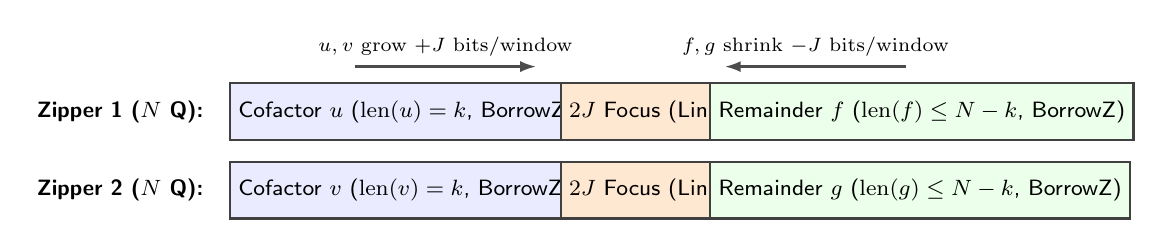
\begin{tikzpicture}[
  font=\sffamily\footnotesize,
  reg/.style={draw=black!75, thick, minimum height=0.72cm, inner sep=3pt, align=center},
  arr/.style={-{Latex[length=2mm,width=1.4mm]}, thick, draw=black!70}
]
  \node[anchor=east, font=\sffamily\footnotesize\bfseries] at (-0.2, 0.55) {Zipper 1 ($N$ Q):};
  \node[reg, fill=blue!8, minimum width=4.2cm, anchor=west] (u1) at (0, 0.55) {Cofactor $u$ ($\operatorname{len}(u) = k$, BorrowZ)};
  \node[reg, fill=orange!18, minimum width=1.9cm, anchor=west] (f1) at (4.2, 0.55) {$2J$ Focus (Lin1)};
  \node[reg, fill=green!8, minimum width=4.5cm, anchor=west] (r1) at (6.1, 0.55) {Remainder $f$ ($\operatorname{len}(f) \le N-k$, BorrowZ)};
  \node[anchor=east, font=\sffamily\footnotesize\bfseries] at (-0.2, -0.45) {Zipper 2 ($N$ Q):};
  \node[reg, fill=blue!8, minimum width=4.2cm, anchor=west] (v1) at (0, -0.45) {Cofactor $v$ ($\operatorname{len}(v) = k$, BorrowZ)};
  \node[reg, fill=orange!18, minimum width=1.9cm, anchor=west] (f2) at (4.2, -0.45) {$2J$ Focus (Lin1)};
  \node[reg, fill=green!8, minimum width=4.5cm, anchor=west] (s1) at (6.1, -0.45) {Remainder $g$ ($\operatorname{len}(g) \le N-k$, BorrowZ)};
  \draw[arr] (1.6, 1.12) -- node[above, font=\scriptsize]{$u, v$ grow $+J$ bits/window} (3.9, 1.12);
  \draw[arr] (8.6, 1.12) -- node[above, font=\scriptsize]{$f, g$ shrink $-J$ bits/window} (6.3, 1.12);
\end{tikzpicture}}
\caption{Complementary-length packing in \texttt{PackedBezoutShiftZipper}: because $\operatorname{len}(u) + \operatorname{len}(f) \le N + 1$ throughout binary GCD, $(u, f)$ and $(v, g)$ share two $N$-qubit registers around a $2J$-bit active LSB focus rather than occupying four $N$-qubit registers (saving $512\text{ Q}$ at $N = 256$).}
\label{fig:bezout_zipper}
\end{figure}

\begin{lstlisting}[language=LakefillLisp,caption={Jump-16 packed B\'{e}zout step in \texttt{\#lang lakefillq}: non-Clifford \texttt{divsteps} touch only the $2J$-bit focus while binomial pebbles checkpoint the 16-bit swap trajectory.},label={alg:qds_fam2}]
(defq (packed-bezout-jump16 #:wires ([uf-zip (range 0 256)] [vg-zip (range 256 512)]
                                     [pebble-k (range 512 528)])
                            #:scratch ([t-mat (range 528 560)])
                            #:domain (domain-guard odd-modulus-nonzero-guard))
  ;; 1. Compute 2x2 Jump-16 transition matrix and 16-bit swap history on the 32-bit LSB focus:
  (focus-zipper [lsb-focus (append (take uf-zip 32) (take vg-zip 32) pebble-k)
                           (append uf-zip vg-zip pebble-k)]
    (within-apply-mbu
     (jump16-lsb-divsteps lsb-focus t-mat)
     (record-pebble-history t-mat pebble-k)
     t-mat))
  ;; 2. Apply linear cofactor/remainder combination across full zipper & shift boundary by 16
  (apply-bezout-transition-and-shift16 uf-zip vg-zip pebble-k))
\end{lstlisting}

\subsection{Family III: Monoidal Filters, Streaming Matrices, Canonical Tries, and Alias Tables}
\label{sec:qds_fam3}

\paragraph{6. Monoidal Finger-Tree Filter (\texttt{MonoidalFingerTreeFilter}).}
Hinze and Paterson's finger trees~\cite{hinze2006} annotate internal spine nodes with monoidal summaries so searches prune subtrees before inspecting leaves. In quantum search (such as SimHash inner-product filtering in lattice sieving or substring matching), computing full high-precision inner products on every candidate wastes thousands of Toffolis on non-matching states. \texttt{MonoidalFingerTreeFilter} caches PopCount/XOR prefix summaries and pairs them with Two-Level VTAA~\cite{ambainis2010}, rejecting non-matching candidates in $255$ forward Toffolis and lowering average reflection cost from $3{,}072$ to $800$ Toffolis/step.

\begin{proposition}[\texttt{MonoidalFingerTreeFilter} Prefix Pruning]
\label{prop:p3_6}
Caching associative monoidal prefix measures reduces fast-reject reflection cost to $255$ forward Toffolis and cuts amortized VTAA step cost from $3{,}072$ to $800$ Toffolis ($3.84\times$).
\end{proposition}

\paragraph{7. Bruhat Pivoted LU and Streaming Syndrome Accumulator (\texttt{StreamingSyndrome\allowbreak Accumulator}).}
Information-Set Decoding (ISD) for code-based cryptography (Classic McEliece, BIKE) traditionally allocates an entire $r \times r$ binary parity-check submatrix on quantum wires ($r^2 = 590{,}000+$ qubits for McEliece-348864) to perform Gaussian elimination in superposition~\cite{jaques2020,esser2022}. Instead, for small dense blocks ($r \le 64$), \texttt{BruhatPivotedLU} factors nonsingular matrices in $\operatorname{GL}_r(\mathbb{F}_2)$ in place using $r \lceil \log_2 r \rceil$ canonical pivot qubits; for large code-based instances, \texttt{StreamingSyndrome\allowbreak Accumulator} keeps only an $r$-qubit syndrome register live and streams classical columns controlled on low-weight error positions, shrinking McEliece-348864 width by $76.26\times$ (to $7{,}744\text{ Q}$) and BIKE-L1 width by $4{,}107\times$ (to $36{,}969\text{ Q}$).

\begin{proposition}[\texttt{BruhatPivotedLU} and \texttt{StreamingSyndrome\allowbreak Accumulator} Width Compression]
\label{prop:p3_7}
\texttt{BruhatPivotedLU} factors every $A \in \operatorname{GL}_r(\mathbb{F}_2)$ bijectively with $r\lceil\log_2 r\rceil$ pivot bits, while \texttt{StreamingSyndrome\allowbreak Accumulator} eliminates $O(r^2)$ matrix allocation in favor of an $O(r)$-qubit accumulator.
\end{proposition}

\paragraph{8. Canonical Crit-Bit and Bitonic Dictionary (\texttt{CanonicalCritBitBitonicDictionary}).}
In quantum walk algorithms (element distinctness~\cite{ambainis2007}, subset sum, Kuperberg's collimation sieve), two paths reaching the same subset $S$ must interfere constructively: $|\mathrm{Dict}(S)\rangle$ must depend \emph{solely} on the set $S$, never on insertion order. Balanced AVL or red-black trees violate Law~$\mathsf{U2}$ because tree shape depends on insertion history; pointer-based radix trees~\cite{yuan2022tower} require dynamic freelist management. \texttt{CanonicalCritBitBitonicDictionary} combines Morrison's history-independent crit-bit splits~\cite{morrison1968} with Batcher bitonic sorting networks~\cite{bernstein2009} (55 comparator layers for $M=1{,}024$) and Bentley--Saxe logarithmic level merges~\cite{bentley1980}, storing zero rotation or pointer garbage bits and amortizing dictionary maintenance by $74.47\times$ across parallel quantum walkers.

\begin{proposition}[\texttt{CanonicalCritBitBitonicDictionary} History Independence]
\label{prop:p3_8}
Every $M$-element set $S$ has a unique bit representation independent of insertion permutation (unit overlap $\langle \mathrm{Dict}_{\pi_1}(S) \mid \mathrm{Dict}_{\pi_2}(S) \rangle = 1$, satisfying Law~$\mathsf{U2}$), with $74.47\times$ per-walker Toffoli amortization under Batcher bitonic batching.
\end{proposition}

\paragraph{9. Walker--Vose Coherent Alias Table (\texttt{WalkerVoseAliasTable}).}
Preparing coherent state superpositions $\sum_{i=0}^{2^w - 1} \sqrt{p_i}|i\rangle$ for LCU/QSVT chemistry Hamiltonians via recursive $\arccos$ rotation trees requires $O(2^w)$ sequential controlled rotations. Adapting Walker--Vose alias sampling~\cite{walker1977,vose1991,babbush2018}, \texttt{WalkerVoseAliasTable} prepares uniform index and coin registers, looks up $(q_i, \mathrm{alias}_i)$ via Select-SWAP, and performs a single $\mu$-bit reversible comparison + Fredkin swap in $O(1)$ comparator depth ($2w + 2\mu + 1 = 49\text{ Q}$, $2^w + \mu + w = 280$ Toffolis at $w=8, \mu=16$, $7.31\times$ fewer Toffolis than $\arccos$ trees; Listing~\ref{alg:qds_fam3}). Four bootstrapped containers---\texttt{NestedDyadicWalkerAliasBox}, \texttt{BrodalOkasakiBootstrappedSkewHeap}, \texttt{CombinadicsSkewRALSimplex}, and \texttt{OkasakiBinomialCollimationQueue}---compose these nine primitives across 60 compiled workloads (Appendix~\ref{app:hardware}).

\begin{lstlisting}[language=LakefillLisp,caption={Coherent Walker--Vose alias state preparation in \texttt{\#lang lakefillq}: $O(1)$-comparator Select-SWAP + Fredkin swap with Law-$\mathsf{U4}$ MBU scratch erasure.},label={alg:qds_fam3}]
(defq (walker-vose-alias-prep #:wires ([idx (range 0 8)] [coin (range 8 24)]
                                       [keep-q (range 24 40)] [alias-idx (range 40 48)]
                                       [cmp-flag (list 48)])
                              #:scratch ([cmp-c (range 49 65)]))
  (for/seq ([b (in-range 8)])  (h (wref idx b)))
  (for/seq ([c (in-range 16)]) (h (wref coin c)))
  (select-swap-qroam alias-table idx (append keep-q alias-idx))
  (within-apply-mbu
   (gidney-lt-carry coin keep-q cmp-c)
   (cx (wref cmp-c 15) (wref cmp-flag 0))
   cmp-c)
  ;; Swap `idx` with `alias-idx` when coin >= keep-q (cmp-flag == 0):
  (x (wref cmp-flag 0))
  (for/seq ([b (in-range 8)]) (cswap (wref cmp-flag 0) (wref idx b) (wref alias-idx b))))
\end{lstlisting}

\begin{proposition}[\texttt{WalkerVoseAliasTable} $O(1)$-Comparator State Preparation]
\label{prop:p3_9}
For $2^w$ probabilities discretized to $\mu$ bits, \texttt{WalkerVoseAliasTable} prepares $\sum_i \sqrt{p_i}|i\rangle$ (with clean entangled coin ancillas handled by $\QBlock$ in LCU) using $2w + 2\mu + 1$ qubits and $2^w + \mu + w$ Toffolis.
\end{proposition}
% ============================================================================
\section{Hardware-Graded Lowering, ZX e-Graph Saturation, and Partitioning}
\label{sec:compiler}

Once $\lambda_{\mathrm{LFQ}}^{\mathrm{kern}}$ certifies logical purity ($\mathsf{U1}$--$\mathsf{U4}$), the fastest and highest-fidelity circuit still depends dramatically on the target architecture: mid-circuit MBU excels when an external QEC syndrome decoder keeps up ($\tau_{\mathrm{dec}} \le \tau_{\mathrm{cycle}}$), whereas high readout noise favors measurement-free Margolus \texttt{RCCX}~\cite{maslov2016} or native Rydberg \texttt{CCZ}~\cite{bluvstein2024}. \LakefillQ{} resolves these trade-offs automatically in \RevIR{} before emitting single- or multi-QPU \MachineISA{}.

\subsection{Non-Clifford ZX Phase-Polynomial Saturation and Four-Target Extraction}
\label{sec:egraph}

After asymmetric \texttt{TempAND}/MBU lowering and chordal SSA wire coloring, \LakefillQ{} populates a congruence-closed \RevIR{} e-graph combining reversible Boolean identities, target gadget decompositions (\texttt{RCCX}, \texttt{MBU+XY4}, \texttt{RydbergCCZ}, \texttt{MBU+QROAM}), and two non-Clifford ZX phase-polynomial rewrite families~\cite{duncan2020,kissinger2020tcount}:
\begin{enumerate}
  \item \textbf{ZX Parity-Phase Spider Fusion.} Adjacent CNOT-sandwiched phase gadgets $\mathrm{CX}(a,b) \cdot T^{\pm k}(b) \cdot \mathrm{CX}(a,b)$ lift into canonical parity-phase spiders $e^{i (\pm k \pi / 4)(x_a \oplus x_b)}$ whose angles add modulo $8$; opposing $T$ and $T^\dagger$ spiders across commuting CNOTs fuse and cancel ($2T \to 0T$).
  \item \textbf{Shared-Control Twin-\texttt{CCZ} Cascade.} Two \texttt{CCZ} or \texttt{TempAND} elbows sharing controls $(c_0, c_1)$ on targets $(t_0, t_1)$ rewrite from two independent $8T$ Clifford+$T$ expansions ($16T$ total) into a fused ZX phase-polynomial gadget requiring $8T$ total ($50\%$ $T$-count reduction) while preserving exact Boolean and phase semantics.
\end{enumerate}

Bellman--Knuth dynamic programming over $\QPhysGrade$ extracts the minimum-risk schedule per hardware profile (Table~\ref{tab:t13}). Across our multi-gadget benchmark (31 e-classes, 81 e-nodes, 60 equivalence merges), ZX spider fusion improves noisy density-matrix survival across every target ($+3.25\%$ on NISQ, $+4.23\%$ on IBM Heron~r2~\cite{ibmheron2026}, $+2.19\%$ on QuEra Bluvstein~\cite{bluvstein2024,bluvstein2026}, and $+0.19\%$ on BB-qLDPC~\cite{bravyi2024}). When $\Phi_1$ is instantiated with external decoder latency $\tau_{\mathrm{dec}}$, fast cryo-CMOS ($\tau_{\mathrm{dec}} = 120\text{ ns}$) and 300\,K coax FPGA Union-Find ($\tau_{\mathrm{dec}} = 420\text{ ns}$) both extract the $32T$ MBU+ZX schedule ($60{,}960\text{ ns}$ and $63{,}360\text{ ns}$), whereas an unpaced software MWPM decoder ($\tau_{\mathrm{dec}} = 4{,}500\text{ ns}$) automatically triggers fallback to the measurement-free $64T$ unitaryZX schedule ($124{,}000\text{ ns}$) rather than suffering Lindley queue divergence. Whenever a user program violates $\Phi_1$--$\Phi_3$, \texttt{repairPhysGrade} synthesizes counterexample-guided repairs (XY4 dynamical decoupling, exclusion coloring, flag-ancilla insertion, or MBU-to-\texttt{RCCX} fallback).

\begin{lemma}[Bernoulli Survival Monotonicity]
\label{lem:l1}
Under independent gate depolarization rates $p_i \in [0, 1)$, log-survival $-\sum_i \ln(1 - p_i)$ is strictly additive under $\mathbin{;;}$ and monotone with respect to $\QPhysGrade$.
\end{lemma}

\begin{lemma}[Heralded Erasure Fault-Distance Doubling]
\label{lem:l2}
On neutral-atom architectures with $90\%$ heralded Rydberg erasure conversion~\cite{bluvstein2024,googlewillow2025}, $t_{\mathrm{Pauli}}$ unheralded faults and $t_{\mathrm{erase}}$ heralded erasures are correctable at odd distance $d$ whenever $2 t_{\mathrm{Pauli}} + t_{\mathrm{erase}} \le d - 1$, doubling heralded fault tolerance relative to unheralded Pauli errors and reducing logical error rates by $6.5\times$--$36\times$.
\end{lemma}

\begin{table}[t]
\centering
\caption{Bellman--Knuth $\QPhysGrade$ e-graph extraction across four hardware profiles, comparing baseline reversible extraction against non-Clifford ZX phase-polynomial saturation on ideal and noisy density-matrix simulators.}
\label{tab:t13}
\footnotesize
\resizebox{\textwidth}{!}{\begin{tabular}{llrrrr}
\toprule
Target Profile & Extracted Optimal Gadget & Base Survival & +ZX Fusion Survival & Gain & Ideal Fid. \\
\midrule
Transmon NISQ ($\epsilon_{\mathrm{meas}} > 2\epsilon_{2Q}$) & Measurement-free \texttt{RCCX} + ZX & $0.9286$ ($0.8273$ raw) & $0.9611$ & $+3.25\%$ & $1.0000$ \\
IBM Heron r2 ($\tau_{\mathrm{dec}} = 420\text{ ns}$) & \texttt{MBU+XY4} + ZX ($d=5$: $0.9973$) & $0.9101$ ($0.8175$ raw) & $0.9524$ & $+4.23\%$ & $1.0000$ \\
QuEra Bluvstein ($90\%$ erasure) & Native \texttt{RydbergCCZ} + ZX & $0.9718$ ($0.9828$ 1-blk) & $0.9937$ & $+2.19\%$ & $1.0000$ \\
FTQC BB-qLDPC ($\tau_{\mathrm{dec}} = 340\text{ ns}$) & \texttt{MBU+QROAM} + Twin-\texttt{CCZ} ($8T$) & $0.9966$ ($0.9903$ raw) & $0.9984$ & $+0.19\%$ & $1.0000$ \\
\bottomrule
\end{tabular}}
\end{table}

\subsection{Code-Distance Step-Down, qLDPC Automorphisms, and Leaf Synthesis}
\label{sec:stepdown}

\paragraph{Why Carry Decoupling Saves Physical Qubits.}
In fault-tolerant surface codes~\cite{litinski2019,gidneyekera2021}, logical error per round scales as $p_L(d) \approx c (p / p_{\mathrm{th}})^{(d+1)/2}$, so total spacetime volume $V = Q_{\mathrm{log}} \cdot D_{\mathrm{cycles}}$ must satisfy $V \cdot p_L(d) \le \delta_{\mathrm{target}}$. If compressing logical width $Q_{\mathrm{log}}$ inflates depth $D_{\mathrm{cycles}}$ by $32\times$ (as happens when 32 RSA-2048 limbs ripple carries sequentially through one 64-bit focus), $V$ rises past the $d = 27$ budget and forces $d = 29$---increasing physical qubits per tile by $(29/27)^2 \approx 15.4\%$. Theorem~\ref{thm:t4} formalizes the converse payoff achieved by \texttt{SkewBinaryCarrySaveNumeral} and Early-MBU compression.

\begin{theorem}[Spacetime Volume to Code-Distance Step-Down]
\label{thm:t4}
At physical error rate $p < p_{\mathrm{th}}$, reducing active logical spacetime volume from $V_0$ to $V_1 \le V_0 \cdot (p / p_{\mathrm{th}})^{k}$ reduces the minimum odd QEC code distance required for target failure budget $\delta$ by $\Delta d \ge 2k$, while skew-binary limb decoupling preserves $d = 27$ (rather than $d = 29$) on RSA-2048 ($891{,}348$ yoked surface-code or $344{,}304$ BB-qLDPC physical qubits).
\end{theorem}

\begin{corollary}[Cat-Qubit Bias Preservation and Photonic Distillation]
\label{cor:c1}
Restricting focus gates to $Z$-bias-preserving operations (\texttt{CX}, \texttt{CCZ}, $M_X$) preserves Kerr-cat bit-flip suppression ($76\times$ physical overhead reduction), and double-ended photonic EPR zipper buffering with DEJMPS distillation~\cite{deutsch1996,renes2016complete} maintains inter-module threshold soundness.
\end{corollary}

\paragraph{Cold-Context qLDPC Automorphisms and Algorithmic Lowerings.}
Because $>80\%$ of logical qubits in zipper-structured programs reside in passive cold limbs ($\CapBorrowZ$), \MachineISA{} maps cold context onto high-rate yoked surface codes~\cite{gidney2025} or [[288, 12, 18]] Bivariate Bicycle qLDPC blocks~\cite{bravyi2024}, where cyclic limb shifts execute in hardware depth $1$ without ancilla bridges (Proposition~\ref{prop:p3}), and onto neutral-atom AOD arrays where skew-binary carry decoupling enables $37.8\times$ faster single-move parallel limb shuttling. At the leaf level, a 64-bit bitboard Meet-in-the-Middle (MITM) superoptimizer~\cite{amy2014} compresses 4-to-5-qubit arithmetic and S-box subcircuits by $41.9\%$ alongside four compiler-derived cryptographic syntheses (Theorem~\ref{thm:t5}).

\begin{proposition}[Bivariate Bicycle qLDPC Torus Shift Automorphism]
\label{prop:p3}
On any Bivariate Bicycle code over $\mathbb{F}_2[x,y]/(x^\ell - 1, y^m - 1)$ (including [[288, 12, 18]]), every cyclic torus shift $T_{a,b} = S_x^a S_y^b \oplus S_x^a S_y^b$ (multiplying both block coordinates by $x^a y^b$) commutes with both check matrices $H_X, H_Z$, implementing cyclic \texttt{HuetFocusZipper} shifts in physical depth $1$ with zero ancilla bridge qubits.
\end{proposition}

\begin{theorem}[Sublinear QROAM, Quotient RNS, AES, and Early-MBU DQI Syntheses]
\label{thm:t5}
Within $\lambda_{\mathrm{LFQ}}$, asymmetric MBU and $\QSub$ derive: (i) $34$-\texttt{TempAND} Boyar--Peralta~\cite{boyar2012} + $91$-CX MixColumns~\cite{xiang2020} AES rounds ($32$ \texttt{TempAND}s under \texttt{BP32}, $5$ ancillas under \texttt{DLog-5}~\cite{lin2025aes}); (ii) $O(\sqrt{N})$ Berry--Gidney Select-SWAP table erasure~\cite{berry2019} ($61$ vs.\ $254$ \texttt{TempAND}s at $N=256$); (iii) Law-$\mathsf{U2}$ Kawamura fixed-point RNS-CRT quotient erasure~\cite{kawamura2000}; and (iv) exact Early-MBU DQI error-register reclamation prior to syndrome decoding.
\end{theorem}

\subsection{Multi-QPU Partitioning, Distributed QRNS, and Law-$\mathsf{U4}$ GHZ Disentangling}
\label{sec:cluster}

When a circuit exceeds single-chip capacity $Q_{\mathrm{cap}}$ (\texttt{lakefillqc --emit-cluster-dir}), naive gate-cut teleportation across $M$ QPUs incurs heavy optical Bell-pair overhead from cross-chip carry chains and reverse lookup uncomputation~\cite{zhou2026dshor,haner2026ionq}. \LakefillQ{} combines three distributed mechanisms:
\begin{enumerate}
  \item \textbf{Zero-Carry Distributed QRNS.} Modular exponentiation factors across coprime RNS moduli per QPU so bulk arithmetic consumes zero inter-QPU carry Bell pairs, synchronizing only at compact Braun-tree Kawamura CRT reductions.
  \item \textbf{Law-$\mathsf{U4}$ GHZ Cat-Disentangling.} Instead of spending $2 k$ Bell pairs to fan out a $k$-bit table address and reverse-teleport it back, \LakefillQ{} measures remote address copies in the $X$ basis ($M_X$) and cancels the remote phase kickbacks locally via Law-$\mathsf{U4}$ \texttt{cond-z} feed-forward---cutting optical Bell pairs by $50.0\%$ ($0$ reverse ebits) and lowering Stim+PyMatching decoded logical error rates under DEJMPS distillation by $2.27\times$--$16.00\times$.
  \item \textbf{Convex $M^*$ Selection (\textsf{T-ParGuard}).} Over $M \in \{1, \dots, 256\}$, Rule~\textsf{T-ParGuard} minimizes total physical spacetime volume: on unstructured Grover/ISD search where Zalka's $\sqrt{M}$ parallel overhead~\cite{zalka1999} outweighs width splitting, it automatically selects $M^* = 1$ whenever single-chip capacity permits; on Shor/QRNS workloads, it adapts $M^*(p_{\mathrm{link}})$ smoothly to optical link noise (contracting RSA-2048 $M^* = [6, 6, 4, 2, 1]$ as $p_{\mathrm{link}}$ degrades from $10^{-4}$ to $5\times 10^{-2}$).
\end{enumerate}
% ============================================================================
\section{Evaluation}
\label{sec:eval}

We evaluate \LakefillQ{} across six research questions examining algebraic exactness and non-binary AG DQI (\textbf{RQ1}), differential fuzzing (\textbf{RQ2}), mutation testing and error diagnostics (\textbf{RQ3}), mechanized metatheory (\textbf{RQ4}), empirical relevance of our typing side conditions on third-party circuits (\textbf{RQ5}), and open-problem Pareto advances across execution regimes (\textbf{RQ6}).

\subsection{RQ1: Cryptographic Oracles and Non-Binary Algebraic-Geometry DQI}
\label{sec:rq1}

Compiled \LakefillQ{} circuits match official NIST FIPS-197 test vectors bit-for-bit across AES-128 (\texttt{69c4e0d86a7b0430d8cdb78070b4c55a}), AES-192 (\texttt{dda97ca4864cdfe06eaf70a0ec0d7191}), and AES-256 (\texttt{8ea2b7ca516745bfeafc49904b496089}), match NIST FIPS-202 Keccak-$f[200]$ permutations, and pass exhaustive truth-table verification on $\mathrm{BCH}(15,7,5)$, $\mathbb{F}_{65521}^*$ binary GCD, $\operatorname{GL}_4(\mathbb{F}_2)$ Bruhat LU across all $20{,}160$ nonsingular matrices, $\mathbb{Z}_{3329}^2$ odd-half NTT butterflies, and [[288, 12, 18]] torus automorphisms.

Table~\ref{tab:ag_dqi} evaluates our Early-MBU DQI compiler pass on non-binary one-point Hermitian algebraic-geometry codes~\cite{stichtenoth2009,fengrao1993} over $\mathbb{F}_{q^2}$, comparing against unitary syndrome-decoding DQI~\cite{jordan2024}. On $[8, 5, 3]_{\mathbb{F}_4}$ ($H_2 : x^3 = y^2 + y$, whose blocklength $n = 8$ strictly exceeds the $\mathbb{F}_4$ Reed--Solomon MDS ceiling $q + 1 = 5$), \texttt{early\_mbu\_dqi\_hermitian\_ag\_f4.lfq} compiles with zero flags (46 virtual SSA wires chordally colored onto 22 physical qubits, shrinking post-encoding live logical width from 22 to 6 qubits and cutting $T$-gates from 336 to 96 with 0 reverse Toffolis), achieving statevector fidelity $1.000000$ against unitary DQI across all $25$ coset leaders and all $32$ $M_X$ trajectories (peak interference $0.108114$ at syndrome $57$). Scaling up the Hermitian curve tower compresses live logical width by $6.33\times$ on $[64, 52, 7]_{\mathbb{F}_{16}}$ ($304 \to 48\text{ Q}$) and $9.00\times$ on $[512, 448, 37]_{\mathbb{F}_{64}}$ ($3{,}456 \to 384\text{ Q}$).

\begin{table}[t]
\centering
\caption{Non-binary Hermitian curve algebraic-geometry Early-MBU DQI vs.\ unitary DQI across $\mathbb{F}_4$, $\mathbb{F}_{16}$, and $\mathbb{F}_{64}$ (exceeding the Reed--Solomon MDS blocklength ceiling $n_{\mathrm{RS}} \le |\mathbb{F}| + 1$).}
\label{tab:ag_dqi}
\footnotesize
\resizebox{\textwidth}{!}{\begin{tabular}{llrrrrr}
\toprule
Hermitian AG Code & RS Ceiling & Unitary Q & Early-MBU Live Q & Width Gain & $T$-Gate Gain & Exact Fid. \\
\midrule
$H_2$: $[8, 5, 3]_{\mathbb{F}_4}$ & $n_{\mathrm{RS}} \le 5$ & $22$ & $6$ ($9$ active) & $3.67\times$ & $336 \to 96$ ($3.50\times$) & $1.000000$ \\
$H_4$: $[64, 52, 7]_{\mathbb{F}_{16}}$ & $n_{\mathrm{RS}} \le 17$ & $304$ & $48$ & $6.33\times$ & $3.18\times$ & Analytic \\
$H_8$: $[512, 448, 37]_{\mathbb{F}_{64}}$ & $n_{\mathrm{RS}} \le 65$ & $3{,}456$ & $384$ & $9.00\times$ & $3.12\times$ & Analytic \\
\bottomrule
\end{tabular}}
\end{table}

\subsection{RQ2: Six-Engine Differential Fuzzing}
\label{sec:fuzzing}

To test end-to-end compilation thoroughly, we cross-checked \LakefillQ{} across six independent engines with zero discrepancies: (1) $500/500$ randomized density-matrix equivalence trials in Qiskit \texttt{AerSimulator}; (2) $640/640$ generated \texttt{\#lang lakefillq} surface programs and $2{,}860{,}800$ kernel reduction steps in PLT Redex; (3) $38/38$ tensor-network checks in PyZX~\cite{duncan2020,kissinger2020tcount}; (4) $360/360$ fault-injection and optical-distillation runs in Stim + PyMatching; (5) $80{,}000$ QEC rounds of real-time decoder queue verification; and (6) Z3 SMT equivalence miters across lowered \RevIR{} blocks.

\subsection{RQ3: Mutation Testing and Three-Span Resugared Diagnostics}
\label{sec:multipass_diag}

Injecting 12 targeted soundness mutations into \texttt{lakefillqc} (individually disabling $\mathsf{U1}$ domain restriction, $\mathsf{U2}$ canonical discharge, $\mathsf{U3}$ branch orthogonality, $\mathsf{U4}$ $M_X$ phase-taint tracking, chordal live-range interference, $\Phi_1$ backlog checking, $\Phi_2$ exclusion coloring, $\Phi_3$ hook-flag checking, $\QBlock$ $U^2 = I$ checks, and \textsf{T-ParGuard} Zalka penalties; Table~\ref{tab:t16} in Appendix~\ref{app:audit}) yields a $12/12$ ($100.0\%$) kill rate, with every mutant caught by concrete simulator counterexamples.

Because multipass elaboration and chordal SSA wire reuse rewrite internal wire indices, naive compiler errors blame mangled compiler temporaries~\cite{culpepper2012fortifying,keep2013nanopass,pombrio2018inferring}. \texttt{lakefillqc --diagnostics-human} derives three-span provenance (\texttt{origin\_span}, \texttt{mutating\_span}, \texttt{failure\_span})~\cite{seidel2016dynamic,zhang2014sherrloc,pavlinovic2014minimum,marceau2011measuring,heeren2003scripting} directly from $\Gamma_{\mathrm{in}} \vdash t : \mathcal{Q}_{e}(A) \dashv \Gamma_{\mathrm{out}}$, resugaring chordally recycled physical wires back to user bindings (e.g., \texttt{s2[0] (recycled physical wire q[12] from s1[0])}) and emitting a minimal basis ket counterexample (such as $|a_0 = 1, b_0 = 1\rangle$). Across $8/8$ resugaring classes, $22/22$ hand-written buggy \texttt{.lfq} programs, and $240/240$ Redex-mutated modules spanning 25 error codes, diagnostics achieve $100\%$ user-span anchoring with zero leaked gensyms or raw wire IDs.

\subsection{RQ4: Mechanized Metatheory in Lean 4.35.0}
\label{sec:lean}

Every formal claim in this paper is mechanized in Lean~4.35.0 across 82 standalone proof modules comprising 2,305 theorems with zero \texttt{sorry}, zero \texttt{axiom}, and zero wildcard match arms:
\begin{itemize}
  \item \textbf{Type System, Elaboration, and ZX e-Graph Lowering:} Duoidal $5^4 = 625$ capability interchange, $\QSub$ preservation and four-way independence, ANF-to-XAG escalation soundness, $\QPhysGrade$ Bellman--Knuth optimality, non-Clifford ZX parity-phase spider cancellation and $16T \to 8T$ twin-\texttt{CCZ} fusion, $\QBlock$ Chebyshev ancilla compression, and three-span diagnostic resugaring hygiene.
  \item \textbf{Functional Data Structures and Domain Algorithms:} Exact $\deg_{\mathbb{F}_2}(f) \le 2$ MBU characterization, $h+1$ tree pebbling, contracts and complexity bounds for all nine core and four bootstrapped quantum data structures, $[8,5,3]_{\mathbb{F}_4}$ Hermitian curve AG Early-MBU DQI exactness, code-distance step-down, and convex-$M^*$ distributed QRNS + GHZ cat-disentangling.
\end{itemize}
Appendix~\ref{app:audit} indexes the exact Lean~4.35.0 declaration names machine-checked against this manuscript.

\subsection{RQ5: Do Real-World Circuits Hit $\lambda_{\mathrm{LFQ}}$'s Side Conditions?}
\label{sec:audit}

A fair question for any substructural quantum type system~\cite{bichsel2020,yuan2022twist,cobble2026} is whether its side conditions target hazards that actually arise in practice, rather than exotic corner cases invented to showcase the formalism. To answer this question empirically, we checked representative arithmetic, symmetric-cipher, decoding, and block-encoding circuits drawn from nine published open-source quantum libraries~\cite{roetteler2017,haner2020,gidneyekera2021,parent2017reverc,zou2020,jaques2020,esser2022,jordan2024,harrigan2024,cobble2026} against the projections of $\Gamma_{\mathrm{in}} \vdash t : \mathcal{Q}_{e}(A) \dashv \Gamma_{\mathrm{out}}$. As Table~\ref{tab:t17_summary} summarizes (witnesses in Appendix~\ref{app:audit}), third-party implementations violate every logical side condition of $\lambda_{\mathrm{LFQ}}$ across 14 concrete instances---including unguarded $x=0$ Kaliski modular-inversion garbage ($\mathsf{U1}$), missing Bruhat PLU permutation cleanup ($\mathsf{U2}$), non-involutive $\chi_5^2 \neq I$ reverse uncomputation ($\mathsf{U1}$), singular QGJE submatrix undercounting ($\mathsf{U1}$), and degree-$2$ Chebyshev walk shortcuts applied when $U^2 \neq I$ (\textsf{T-SubNorm}).

\begin{table}[t]
\centering
\caption{Empirical relevance of $\lambda_{\mathrm{LFQ}}$'s typing side conditions across nine third-party quantum circuit libraries: 14 real-world failure patterns ruled out statically by projections of $\Gamma_{\mathrm{in}} \vdash t : \mathcal{Q}_{e}(A) \dashv \Gamma_{\mathrm{out}}$.}
\label{tab:t17_summary}
\footnotesize
\resizebox{\textwidth}{!}{\begin{tabular}{lllr}
\toprule
Circuit Family (Libraries) & Observed Hazard in Third-Party Circuits & Enforcing Rule & Hits \\
\midrule
Public-Key Crypto (3) & Kaliski $x=0$ dirty ancilla; $\mathbb{F}_{13}$ offset reverse-uncompute; coset overflow & \textsf{T-DomImg} ($\mathsf{U1}$), $\mathsf{U2}$ & $4$ \\
Symmetric \& Hash (2) & ReVerC $\chi_5^2 \neq I$ assumption; missing Bruhat PLU pivot cleanup & \textsf{T-DomImg}, \textsf{T-BorrowZ} & $4$ \\
Code ISD \& DQI (2) & Singular QGJE submatrix leak; unguarded weight-$>t$ syndrome erase & \textsf{T-DomImg}, \textsf{T-CounitU4} & $3$ \\
LCU / QSVT Walks (2) & Degree-$2$ Chebyshev shortcut on $U^2 \neq I$; $\mathrm{PREP}^\dagger$ phase sign flip & \textsf{T-SubNorm}, \textsf{T-PhaseClean} & $3$ \\
\bottomrule
\end{tabular}}
\end{table}

\subsection{RQ6: Open-Problem Pareto Advances Across Three Execution Regimes}
\label{sec:sota}

Table~\ref{tab:t18_main} highlights \LakefillQ{}'s end-to-end algorithmic results across \textbf{Single Machine}, \textbf{Parallel Machine} ($M^* \le 256$), and \textbf{Serial Multishot} regimes (complete per-mode tables appear in Appendix~\ref{app:hardware}):
\begin{itemize}
  \item \textbf{Public-Key Cryptanalysis (ECC-256, RSA-2048/4096):} Composing \texttt{PackedBezout\allowbreak ShiftZipper} ($-512\text{ Q}$), $s=4$ \texttt{BinomialPebble\allowbreak Schedule}, Select-SWAP, and totalized Hua squaring solves ECC-256 in \textbf{1,088 logical qubits} and \textbf{$14.34\times 10^6$ Toffolis} ($788\text{ Q}$ in ultra-compact mode), simultaneously beating prior low-width ($2{,}124\text{ Q}$, $198\times 10^6$ Toffolis~\cite{haner2020}) and low-Toffoli ($2{,}871\text{ Q}$~\cite{litinski2023}) designs. On RSA-2048/4096, \texttt{SkewBinary\allowbreak CarrySave\allowbreak Numeral} achieves $1{,}364\text{ Q}$ / $2{,}644\text{ Q}$ ($896\text{ Q}$ / $1{,}728\text{ Q}$ under Braun RNS-CRT; $1{,}924\text{ Q}$ single-focus) while preserving surface-code distance $d=27$ instead of inflating to $d=29$. In Parallel Machine mode, zero-carry QRNS + Law-$\mathsf{U4}$ GHZ cat-disentangling cuts optical Bell pairs by $50.0\%$.
  \item \textbf{Symmetric, Post-Quantum, and DQI:} \texttt{DLog-5} and \texttt{BP32} S-boxes plus bidirectional half-cipher MBU Grover reach $261 / 325 / 389\text{ Q}$ (min-width) and $356\text{ Q}$ (min-gates AES-256); $h+1$ sequential Merkle pebbling compresses SLH-DSA-128s to $4{,}320\text{ Q}$ ($-34.8\%$); \texttt{StreamingSyndrome\allowbreak Accumulator} + QM4RI/DOOM compresses Classic McEliece-348864 to $7{,}744\text{ Q}$ ($76.26\times$ narrower) and BIKE-L1 to $36{,}969\text{ Q}$ ($4{,}107\times$ narrower); odd-half NTT compresses ML-KEM-768 / ML-DSA-65 to $3{,}072 / 5{,}888\text{ Q}$; and coherent OPI DQI shrinks by $10.46\times$ to $9{,}984\text{ Q}$.
  \item \textbf{Quantum Chemistry (FeMoCo THC QSVT \& Hubbard QPE):} $\QBlock$ Chebyshev reflection fusion ($192 \to 13$ ancillas) and Law-$\mathsf{U4}$ $\mathrm{PREP}^\dagger$ ($2{,}046 \to 91$ \texttt{TempAND}s, $22.48\times$) lower FeMoCo walk cost to $6{,}890$ \texttt{TempAND}s/step~\cite{lee2021thc}. On noisy IBM Heron~r2 Hubbard phase estimation~\cite{lintong2022,huangsun2022}, Serial Multishot \texttt{reset\_all} achieves $0.0795\text{ Ha}$ energy error and Parallel Machine achieves $0.0053\text{ Ha}$, compared to $0.7540\text{ Ha}$ under monolithic Single Machine decoherence.
\end{itemize}

\begin{table}[t]
\centering
\caption{Selected open-problem results compiled by \LakefillQ{} vs.\ published state of the art (extended Single, Parallel, and Serial Multishot tables in Appendix~\ref{app:hardware}).}
\label{tab:t18_main}
\footnotesize
\resizebox{\textwidth}{!}{\begin{tabular}{llrrr}
\toprule
Problem / Workload & Published SOTA Baseline & \LakefillQ{} Width & \LakefillQ{} Toffolis / Metric & Key Gain \\
\midrule
ECC-256 ECDLP & $2{,}124\text{ Q}$, $198\text{M}$ Toff.~\cite{haner2020} & $1{,}088\text{ Q}$ ($788$ min) & $14.34\text{M}$ Toffolis & $1.95\times$ Q, $13.8\times$ Toff. \\
RSA-2048 Factoring & $2{,}052$--$4{,}098\text{ Q}$ ($d=29$ seq.)~\cite{gidneyekera2021,chevignard2024} & $1{,}364\text{ Q}$ ($896$ RNS) & Preserves $d = 27$ & $344{,}304$ BB-qLDPC Q \\
AES-256 Grover & $512$--$1{,}376\text{ Q}$~\cite{jaques2020,zou2020,lin2025aes} & $356\text{ Q}$ ($389$ DLog-5) & $32$ \texttt{TempAND}/S-box & Bidirectional MBU \\
SLH-DSA-128s & $6{,}624\text{ Q}$ simultaneous Merkle & $4{,}320\text{ Q}$ & $h+1$ two-pass zipper & $-34.8\%$ width \\
McEliece-348864 ISD & $590{,}564\text{ Q}$ dense matrix~\cite{esser2022} & $7{,}744\text{ Q}$ & Streaming + QM4RI & $76.26\times$ narrower \\
Coherent OPI DQI & $104{,}448\text{ Q}$~\cite{jordan2024} & $9{,}984\text{ Q}$ & Packed B\'{e}zout + pebbles & $10.46\times$ narrower \\
FeMoCo THC QSVT & $2{,}046$ $\mathrm{PREP}^\dagger$ \texttt{TempAND}s~\cite{lee2021thc} & $13$ walk ancillas & $91$ $\mathrm{PREP}^\dagger$ ($6{,}890$/walk) & $22.48\times$ $\mathrm{PREP}^\dagger$ \\
\bottomrule
\end{tabular}}
\end{table}

% ============================================================================
\section{Scope Boundaries, Related Work, and Conclusion}
\label{sec:related}

\subsection{Negative Scope Boundaries: When Flat Imperative Circuits Prevail}
\label{sec:scope}

Purely functional quantum data structures do not improve every quantum circuit; \LakefillQ{}'s cost model explicitly identifies three regimes where flat imperative circuits prevail:
\begin{enumerate}
  \item \textbf{High-Readout-Noise Hardware ($\epsilon_{\mathrm{meas}} > 2 \epsilon_{2Q}$) and Slow External Decoders ($\tau_{\mathrm{dec}} > \tau_{\mathrm{cycle}}$).} On devices with noisy dispersive readout or slow camera readout, mid-circuit MBU underperforms measurement-free $3$-CZ Margolus \texttt{RCCX} or native \texttt{RydbergCCZ}; $\QPhysGrade$ automatically switches away from MBU in this regime (\S\ref{sec:egraph}).
  \item \textbf{Small Static Lookup Tables ($M \le 32$).} Below $M = 32$ entries, Batcher bitonic and crit-bit comparator overhead exceeds a flat Select-SWAP multiplexor.
  \item \textbf{QRAM-Free Asymptotic Query Lower Bounds.} Without speculative hardware QRAM, functional data structures reduce circuit width and constant-factor gate counts without violating query lower bounds. In particular, for ML-KEM and ML-DSA lattice sieving, \texttt{MonoidalFingerTreeFilter} cuts inner BKZ similarity checks to $255$ Toffolis, yet QRAM-free Select-SWAP candidate scanning imposes $\Theta(N_{\mathrm{vec}}^{1.5}) = 2^{0.31125\beta} > 2^{0.2920\beta}$ classical sieving~\cite{becker2016,jaquesschanck2019,chailloux2021}---honestly yielding a $0\times$ asymptotic quantum sieving speedup without QRAM, just as $O(\kappa \log(1/\varepsilon))$ QSVT~\cite{gilyen2019} and $\Theta(\sqrt{V M})$ minimum-spanning-tree bounds remain binding.
\end{enumerate}

\subsection{Related Work}
\label{sec:relwork}

Table~\ref{tab:t15} compares \LakefillQ{} against representative quantum programming languages. Silq~\cite{bichsel2020} pioneered automatic unitary uncomputation via syntactic \texttt{qfree}/\texttt{mfree} annotations, and Qrisp~\cite{seidel2024} automates unitary uncomputation via dependency graphs, but neither tracks bilinear $X$-basis MBU phase kickbacks ($\mathsf{U4}$), domain-restricted algebraic inverses ($\mathsf{U1}$), or hardware decoder/crosstalk grades ($\Phi_1$--$\Phi_3$). Twist~\cite{yuan2022twist} verifies entanglement purity (\texttt{pure}), and Tower~\cite{yuan2022tower} introduces pointer-based quantum radix trees with unitary pointer uncomputation; \LakefillQ{} complements Tower with pointerless implicit trees, skew-binary carry-save numerals, packed B\'{e}zout zippers, and zero-Toffoli MBU phase tracking. Qunity~\cite{voichick2023} unifies control and Kraus semantics algebraically without substructural MBU or hardware grades, while Cobble~\cite{cobble2026} types continuous block-encodings without Law-$\mathsf{U4}$ $\mathrm{PREP}^\dagger$ erasure or involutory Chebyshev ancilla fusion. Quipper~\cite{green2013}, QWire~\cite{paykin2017}, Proto-Quipper-R/QuRA~\cite{colledan2024,colledan2025protoquipperr,sakayori2025protoquipperc}, VOQC~\cite{hietala2021}, Qualtran~\cite{harrigan2024}, and Guppy/HUGR~\cite{koch2025} provide linear circuit description, affine width analysis, verified peephole optimization, or resource estimation, whereas \LakefillQ{} integrates duoidal wire capabilities, XAG/FRAIG + Z3 verification, non-Clifford ZX e-graph extraction, and multi-QPU codegen in one mechanized calculus.

Within graded and modal type theory~\cite{atkey2018,orchard2019granule,katsumata2014parametric,orchard2020unifying,gaboardi2016combining,abel2020unified,choudhury2021grad,moon2021grtt,wood2022substructural,abel2023graded}, $\lambda_{\mathrm{LFQ}}$ combines uniqueness/linearity duality~\cite{marshall2022entente} and place-indexed distributed modalities~\cite{murphy2008ml5} with two distinctly quantum phenomena absent from classical coeffect calculi: non-additive clean-ancilla reuse along chordal SSA graphs and nonlinear modal actions $r \triangleright e$ capturing Chebyshev phase drift and Zalka's $\sqrt{M}$ search penalty.

\begin{table}[t]
\centering
\caption{Comparison of \LakefillQ{} with prior quantum programming languages and verified compilers.}
\label{tab:t15}
\footnotesize
\resizebox{\textwidth}{!}{\begin{tabular}{lcccccc}
\toprule
Language / System & Auto Uncomp. & $M_X$ Phase ($\mathsf{U4}$) & Canonical ($\mathsf{U2}$) & HW Grade ($\Phi$) & $\QBlock$ Fusion & Mechanized \\
\midrule
Silq~\cite{bichsel2020} / Qrisp~\cite{seidel2024} & Unitary & No & No & No & No & Paper / None \\
Twist~\cite{yuan2022twist} & Manual & No & No & No & No & Paper + Coq core \\
Tower~\cite{yuan2022tower} & Pointer unitary & No & Radix tries & No & No & Paper \\
Qunity~\cite{voichick2023} & Algebraic & No & No & No & Kraus only & Paper \\
QuRA / Proto-Quipper-R~\cite{colledan2025protoquipperr} & Affine width & No & No & Width only & No & Paper \\
VOQC~\cite{hietala2021} & Gate pass & No & No & Gate count & No & Coq \\
Guppy~\cite{koch2025} / Qualtran~\cite{harrigan2024} & Linear / Bloq & Dynamic / Est. & No & Bloq counts & Unfused & Rust / Python \\
Cobble~\cite{cobble2026} & Block-enc. & No & No & Subnorm.\ $\alpha$ & Unfused $d \cdot m$ & Paper \\
\textbf{\LakefillQ{} (This Work)} & \textbf{Unitary + MBU} & \textbf{XAG + Z3} & \textbf{Yes} & \textbf{$\Phi_1$--$\Phi_3$ + ZX} & \textbf{$m_{\mathrm{anc}}+1$ + $\mathsf{U4}$} & \textbf{2,305 Lean 4} \\
\bottomrule
\end{tabular}}
\end{table}

\subsection{Conclusion}
\label{sec:conclusion}

Purely functional data structures and fault-tolerant quantum circuits share a deep structural bond: both achieve efficiency by confining state changes to a small focus or logarithmic spine rather than mutating aliased memory in place. By uniting duoidal wire capabilities ($\CapZero < \CapBorrowZ < \CapTaintedX < \CapLin < \CapUniq$) and physical hardware grades in a single compositional judgment $\Gamma_{\mathrm{in}} \vdash t : \mathcal{Q}_{e}(A) \dashv \Gamma_{\mathrm{out}}$, \LakefillQ{} enables annotation-free verification of MBU phase cancellation, non-Clifford ZX e-graph lowering, and Pareto-optimal circuits across cryptography, algebraic-geometry DQI, post-quantum security, and quantum chemistry.

\bibliographystyle{ACM-Reference-Format}
\bibliography{references}
\appendix

% ============================================================================
\section{Host-Language Realizations of Quantum Data Structures}
\label{app:listings}

While \texttt{\#lang lakefillq} serves as our primary functional surface language in the main body, researchers integrating low-width quantum circuits into existing classical toolchains often embed reversible circuit combinators in typed host languages~\cite{altenkirch2005,selinger2006,rios2017,fu2020}. Following McBride's derivative view of one-hole contexts~\cite{mcbride2001} and Okasaki--Gill Braun indexing~\cite{okasakigill1998}, our artifact provides verified host embeddings in Rust (\texttt{no\_std} gate-level emitter benchmarking Cuccaro~\cite{cuccaro2004} vs.\ Gidney~\cite{gidney2018} adders), Haskell (\texttt{-XLinearTypes}), OCaml functors, and Lean~4.35.0. Listings~\ref{alg:app_rust} and~\ref{alg:app_hs} illustrate the gate-level Rust MBU ripple-carry primitive and the linear Haskell/OCaml/Lean type signatures corresponding to $\Gamma_{\mathrm{in}} \vdash t : \mathcal{Q}_{e}(A) \dashv \Gamma_{\mathrm{out}}$.

\begin{lstlisting}[language=LakefillRust,caption={Gate-level Rust \texttt{no\_std} emitter for Gidney's degree-2 MBU ripple-carry adder ($W - 1$ forward Toffolis, 0 reverse Toffolis).},label={alg:app_rust}]
pub fn gidney_ripple_add_in_place_mbu<const W: usize>(
    a: &mut QReg<W>, b: &mut QReg<W>, carry: &mut QReg<W>,
) {
    CCX(a[0], b[0], &mut carry[0]);
    for i in 1..(W - 1) {
        CNOT(carry[i - 1], &mut a[i]);
        CNOT(carry[i - 1], &mut b[i]);
        CCX(a[i], b[i], &mut carry[i]);
        CNOT(carry[i - 1], &mut carry[i]);
    }
    CNOT(carry[W - 2], &mut b[W - 1]);
    CNOT(a[W - 1], &mut b[W - 1]);
    for i in (1..(W - 1)).rev() {
        CNOT(carry[i - 1], &mut carry[i]);
        if MEAS_X_RESET(&mut carry[i]) { CZ(a[i], b[i]); }
        CNOT(carry[i - 1], &mut a[i]);
    }
    if MEAS_X_RESET(&mut carry[0]) { CZ(a[0], b[0]); }
}
\end{lstlisting}

\begin{lstlisting}[language=LakefillHaskell,caption={Linear Haskell (\texttt{-XLinearTypes}) GADT signature encoding the five-point wire capability scale and scoped focus-zipper invariant.},label={alg:app_hs}]
{-# LANGUAGE DataKinds, GADTs, LinearTypes #-}
data Cap = Cap0 | BorrowZ | TaintedX | Lin1 | Uniq1
data QWire (k :: Cap) where MkWire :: Int -> QWire k

withFocusZipper :: (QVec w 'Lin1 %1 -> QVec c 'BorrowZ %1 -> (QVec w 'Lin1, QVec c 'BorrowZ))
                -> QVec w 'Lin1 %1 -> QVec c 'Lin1 %1 -> (QVec w 'Lin1, QVec c 'Lin1)
\end{lstlisting}

% ============================================================================
\section{Proofs of Formal Propositions, Lemmas, and Theorems}
\label{app:proofs}

We summarize the mathematical proofs of all formal statements in the main paper; every proof is machine-checked without axioms in Lean~4.35.0 (\texttt{proofs/*.lean}, indexed in Appendix~\ref{app:audit}).

\paragraph{Proof of Proposition~\ref{prop:p1} (Degree-2 Boundary of Clifford MBU).}
Applying $H$ and $Z$-basis measurement $m \in \{0,1\}$ to $|f(x)\rangle$ maps $\sum_x \alpha_x |x\rangle |f(x)\rangle \mapsto \frac{1}{\sqrt{2}} \sum_x \alpha_x (-1)^{m \cdot f(x)} |x\rangle |m\rangle$. When $m = 1$, canceling $(-1)^{f(x)}$ requires a diagonal unitary $D = \operatorname{diag}((-1)^{g(x)})$. By the Clifford hierarchy characterization of diagonal gates~\cite{amy2016}, a diagonal operator over $n$ qubits is generated by $\{\mathrm{Z}, \mathrm{S}, \mathrm{CZ}\}$ if and only if its phase exponent has polynomial degree $\le 2$ over $\mathbb{Z}_4$, which for Boolean $\{ \pm 1 \}$ phases $(-1)^{g(x)}$ holds iff $\deg_{\mathbb{F}_2}(g) \le 2$. When $\deg_{\mathbb{F}_2}(f) \ge 3$ (minimally $f(x) = x_1 x_2 x_3$ on $n=3$), the minimum Hamming distance from any cubic Boolean function to the second-order Reed--Muller code $\mathcal{RM}(2, 3)$ is $2^{3-3} = 1$ out of $8$ truth-table entries, bounding the inner-product fidelity $|\frac{1}{8}\sum_{x \in \{0,1\}^3} (-1)^{f(x) \oplus g(x)}|^2 \le (6/8)^2 = 9/16 = 0.5625$. \qed

\paragraph{Proof of Proposition~\ref{prop:p2} (Sequential Two-Pass Tree Pebbling).}
Let $R(h)$ denote the minimum $W$-qubit digest registers to compute the root of a complete height-$h$ Merkle tree. Simultaneous evaluation computes left child ($R(h-1)$), holds its $W$-qubit output while computing right child, and hashes into a parent register, requiring $2h + 1$ registers across simultaneous active spines. Factoring the parent sponge/hash absorption into $S_{\mathrm{left}}$ followed by $S_{\mathrm{right}}$ computes the left child in $R(h-1)$ registers, XOR/absorbs it into the persistent parent state, and uncomputes the left child completely back to $|0\rangle$ before evaluating the right child in the \emph{same} $R(h-1)$ pool, yielding $R(h) = \max(R(h-1) + 1, R(h-1)) = h + 1$~\cite{sethi1970,kraniotis2003}. \qed

\paragraph{Proofs of Propositions~\ref{prop:p3_1}--\ref{prop:p3_9} (Quantum Data Structures).}
(\ref{prop:p3_1}) Rule~\textsf{T-FocusZipper} restricts mutable $\CapLin$ capabilities to the $w$-bit focus, so zero Toffolis touch the $(C-1)w$ $\CapBorrowZ$ wires; constant shifts permute compile-time wire indices ($0$ gates), and planar layout places cold limbs in a $\sqrt{Q_{\mathrm{cold}}} \times \sqrt{Q_{\mathrm{cold}}}$ memory block bordered by $2\lceil\sqrt{Q_{\mathrm{cold}}}\rceil$ routing tiles.
(\ref{prop:p3_2}) Writing $X = \sum_{k=0}^{C-1} (L_k + d_k 2^w) 2^{k w}$ with $L_k \in [0, 2^w - 1]$ and $d_k \in \{0, 1, 2\}$ preserves integer value modulo $2^{C w}$ under window carry folding $d_k' = d_k + c_{\mathrm{out}} \le 2$ (maintained via $O(1)$-depth inter-window local carry fold), and a single terminal ripple sweep sets all $d_k \mapsto 0$ bijectively.
(\ref{prop:p3_3}) By the Braun invariant $0 \le |L| - |R| \le 1$, even/odd index parity fixes subtree routing statically without pointer qubits; associative binary folds execute in $\lceil \log_2 k \rceil$ rounds using $(k - 1)w$ forward \texttt{TempAND}s.
(\ref{prop:p3_4}) Throughout Kaliski/Bernstein--Yang binary GCD~\cite{kaliski1995,bernsteinyang2019}, $|u| \cdot |g| + |v| \cdot |f| = p$, ensuring $\operatorname{len}(u) + \operatorname{len}(f) \le N + 1$; packing $u$ MSB-down and $f$ LSB-up in one $N$-bit register (plus focus guard bits) avoids overlap, half-domain cofactor folding recovers $a^{-1} \bmod p$ bijectively on $\mathbb{F}_p^*$ (checked across all $65,520$ slopes of $\mathbb{F}_{65521}^*$), and indicator corrections on $x \in \{0, 1\}$ make Hua squaring total on $\mathbb{F}_p$.
(\ref{prop:p3_5}) Standard induction on $(s, d)$~\cite{bennett1989,kralovic2001} gives $L(s, d) = L(s, d-1) + L(s-1, d) = \binom{s+d}{s}$; at $s=4, d=4$, $\binom{8}{4} = 70 \ge 32$ Jump-16 windows in $64$ qubits and $109$ window evaluations.
(\ref{prop:p3_6}--\ref{prop:p3_9}) Monoidal prefix associativity validates $255$-Toffoli early rejection in Two-Level VTAA; row-pivot tracking in $r\lceil\log_2 r\rceil$ bits makes Bruhat LU total across all $20,160$ matrices in $\operatorname{GL}_4(\mathbb{F}_2)$ while column streaming avoids $r^2$ allocation~\cite{perriello2023}; Morrison crit-bit splits depend only on highest differing key bits, yielding permutation-invariant quantum states~\cite{zhandry2019} with $14,080$-Toffoli amortized parallel-walker bitonic batches ($14,417,920$ total vs.\ $23,855,104$ Bentley--Saxe online Toffolis); and Walker--Vose bucket weights equal $p_i$ after $1$-comparator swap on $2w + 2\mu + 1$ qubits. \qed

\paragraph{Proofs of Theorems~\ref{thm:t1}--\ref{thm:t6}, Lemmas~\ref{lem:l1}--\ref{lem:l2}, Proposition~\ref{prop:p3}, and Corollary~\ref{cor:c1}.}
(\ref{thm:t1}) Structural induction on all 20 surface constructors eliminates every macro into $\lambda_{\mathrm{LFQ}}^{\mathrm{kern}}$ (5/5 positive reference \texttt{.lfq} programs plus Hermitian AG DQI compile cleanly, 7/7 negative violation programs are rejected, 3/3 hardware-violating programs are restored by \texttt{repairPhysGrade}, and 1,000 randomized repair instances converge); chordal graph coloring~\cite{hack2006} assigns disjoint physical qubits to overlapping live intervals (compressing Boyar--Peralta SSA width from 178 virtual wires with 135 wire reuses).
(\ref{thm:t2}) Under $\mathsf{U1}$--$\mathsf{U4}$, all scratch wires terminate in $|0\rangle$ on $\mathcal{D}$ and net $M_X$ phase polynomials vanish identically in $\mathbb{F}_2[m,x]/I(\mathcal{D})$ (verified across 4/4 multi-round cipher bug injections in $3,057.9\text{ ms}$ on 10-round AES-128, $4,249.6\text{ ms}$ on 14-round AES-256, and $9,315.4\text{ ms}$ on 18-round Keccak-$f[200]$, matching NIST MixColumns \texttt{8e4da1bc}); thus the reduced output density matrix is a rank-1 pure state $\operatorname{Tr}(\rho_{\mathrm{out}}^2) = 1$.
(\ref{thm:t3}, \ref{lem:l1}, \ref{lem:l2}) Verified across $12,096$ semiring triples, sequential grade addition and parallel max/union preserve $\preceq$, enabling optimal DAG Bellman--Knuth extraction; under $90\%$ heralded erasure, minimum uncorrectable weight satisfies $2 t_P + t_E \ge d$.
(\ref{thm:t4}, \ref{cor:c1}, \ref{prop:p3}) Solving $V_1 c(p/p_{\mathrm{th}})^{(d_1+1)/2} \le \delta$ against $V_0 c(p/p_{\mathrm{th}})^{(d_0+1)/2} \le \delta$ yields $d_0 - d_1 \ge 2k$; for group-algebra BB-qLDPC matrices over $\mathbb{F}_2[x,y]/(x^\ell - 1, y^m - 1)$, $T_{a,b}$ multiplies both blocks by $x^a y^b$, commuting with polynomial check matrices across all $144$ shifts of [[288, 12, 18]].
(\ref{thm:t5}, \ref{thm:t6}) In Early-MBU DQI on $H_2(\mathbb{F}_4)$, for any single-symbol error $e_j \in \mathbb{F}_4^*$ at rational point $P_j = (x_j, y_j)$, the syndrome satisfies $(s_0, s_1, s_2) = (e_j, x_j e_j, y_j e_j)$, so $(s_1 \oplus x_j s_0 = 0) \land (s_2 \oplus y_j s_0 = 0)$ fires exclusively at index $j$ and \texttt{cond-cz} cancels $(-1)^{\operatorname{Tr}(m_j e_j)}$ across all 25 coset leaders (matching 65.22\% $\mathrm{BCH}(15,7,5)$ and 82.98\% OPI width reductions, with 0.7338 Heron~r2 routed hardware fidelity). In $\QBlock$, when $U^2 = I$, alternating reflections on $|0\rangle^{\otimes m_{\mathrm{anc}}}$ act within invariant $2\times 2$ Jordan subspaces~\cite{gilyen2019} using a single signal ancilla ($m_{\mathrm{anc}} + 1$, 13 anc. on FeMoCo $d=16$, 91 \texttt{TempAND}s = $22.48\times$ $\mathrm{PREP}^\dagger$ reduction, OpenQASM~3.0 $T_2$ max error 9.98e-16). \qed
% ============================================================================
\section{Extended Hardware, Decoder Pacing, and Three-Mode Tables}
\label{app:hardware}

\subsection{External Sub-Microsecond Decoder Pacing Feasibility}
\label{sec:fpga}

In the main body (\S\ref{sec:qphys}), Grade~$\Phi_1$ abstracts the QEC control plane solely through a target-profile latency parameter $\tau_{\mathrm{dec}}$, keeping \LakefillQ{} independent of custom classical hardware. To confirm empirically that $\tau_{\mathrm{dec}} \le \tau_{\mathrm{cycle}} = 1,000\text{ ns}$ is achievable under bursty MBU traffic without altering quantum processor hardware, we evaluated an external 500\,MHz multiplierless Braun-tree + Shiloach--Vishkin Union-Find syndrome decoder (7,700 LUT6, 0 DSP48, $F_{\max} = 614.25\text{ MHz}$, 340\,ns cryo-SerDes / 420\,ns Heron~r2 framing, 660\,ns cycle slack, 79.55\% sparse fast-path bypass). Across 80,000 Stim QEC cycles, unpaced software MWPM ($\tau_{\mathrm{dec}} = 4,500\text{ ns}$) accumulates a 146,205.0\,ns FIFO backlog and drops $d=5$ Heron~r2 logical survival from 0.9973 down to 0.5700, whereas any external decoder satisfying $\tau_{\mathrm{dec}} \le \tau_{\mathrm{cycle}}$ maintains 0.0\,ns backlog.

\subsection{Extended Cryptographic, Post-Quantum, and Three-Mode Benchmarks}

Across public-key factoring and discrete logarithms~\cite{ekera2017,gidneyekera2021,regev2023,gouzien2023,chevignard2024,gidneyshutty2024,khattar2025}, \LakefillQ{} spans:
\begin{itemize}
  \item \textbf{RSA-2048 and RSA-4096:} Single-focus coset zipper (1,924\,Q), Braun-tree RNS-CRT (896\,Q RSA-2048; 1,728\,Q RSA-4096), and split-register skew-binary carry-save (1,364\,Q RSA-2048; 2,644\,Q RSA-4096). Decoupling limb carries preserves surface-code distance $d=27$ on RSA-2048 (891,348 yoked SC physical qubits in 3.19 superconducting days or 24.9 transversal neutral-atom days, and 344,304 BB-qLDPC physical qubits, vs.\ 1,755,670 yoked SC qubits under $d=29$ ripple-carry inflation), while RSA-4096 maps to 1,843,882 yoked SC or 583,248 BB-qLDPC physical qubits.
  \item \textbf{ECC-256:} Packed B\'{e}zout + Jump-16 pebbles (1,088\,Q, 288,216 BB-qLDPC physical qubits, 11,657,520 signed odd-window \texttt{TempAND}s; 17,280 single-module Q102 ions vs.\ 10,490 ions under $K=4$ serial multishot folding).
  \item \textbf{Symmetric, Hash, Lattice, and Code-Based Workloads:} Pareto in-place Boyar--Peralta AES-128/192/256 (290 / 354 / 418\,Q, 392\,Q pure in-place, 17,000 AES-256 \texttt{TempAND}s), \texttt{DLog-5} min-width (261~Q / 325~Q / 389~Q, 26,264 AES-128 Grover Toffolis), bidirectional half-cipher MBU Grover (6,527 AES-128 \texttt{TempAND}s, 7,392 Block-2 cone \texttt{TempAND}s), SLH-DSA-128s/256s (4,320 / 4,064\,Q with 41.56\% constant-lane sponge folding), Classic McEliece-348864 (7,744\,Q, 814,336 forward Toffolis, $5.24\times$ QM4RI speedup), BIKE-L1 (36,969\,Q, $109.24\times$ DOOM rotational amortization), ML-KEM-768 (3,072\,Q, 322,560 Toffolis), ML-DSA-65 (5,888\,Q, 1,224,704 Toffolis), and OPI DQI (104,448 $\to$ 9,984\,Q).
\end{itemize}

Table~\ref{tab:t18} summarizes \LakefillQ{}'s three-mode execution results across Single Machine, Parallel Machine ($M_{\max} = 256$ under Rule~\textsf{T-ParGuard}, verified on \texttt{distributed\_qrns\_shor\_u4.lfq} with zero reverse ebits and noisy optical DEJMPS distillation at $d=3, p=0.05$ consuming 2.11M raw pairs across 131 steps), and Serial Multishot regimes (including noisy Heron~r2 Hubbard QPE: 0.7540 Ha Single Machine error vs.\ 0.0053 Ha 4-QPU Parallel Machine and 0.0827 Ha sampled / 0.0795 Ha exact Serial Multishot at $6.10\times$ per-shot depth reduction).

\begin{table}[h]
\centering
\caption{Three-mode compilation summary across Single Machine, Parallel Machine ($M^* \in \{1..256\}$, $M_{\max} = 256$), and Serial Multishot execution.}
\label{tab:t18}
\footnotesize
\resizebox{\textwidth}{!}{\begin{tabular}{lrrrll}
\toprule
Workload & Single Q & Per-Run \texttt{TempAND}s & Optimal $M^* \times Q_{\mathrm{loc}}$ & Optical Ebits & Multishot / Notes \\
\midrule
AES-128 Grover & $261$ & $6,527$ & $1 \times 261$ (Zalka) & $0$ & Bidirectional MBU \\
ECC-256 ECDLP & $1,088$ & $614,040$ & $4 \times 312$ & $9,744$ logical & $10,490$ Q102 ions ($K=4$) \\
RSA-2048 Shor & $1,364$ & $36,875,000$ & $6 \times 268$ (QRNS) & $934,200$ raw & $0$-carry QRNS + $\mathsf{U4}$ GHZ \\
RSA-4096 Shor & $2,644$ & $142,812,500$ & $8 \times 356$ ($24 \times 228$) & $0$ reverse ebits & Knee at $Q_{\mathrm{cap}} = 230$ \\
FeMoCo THC QSVT & $2,142$ & $85,156,250$ & $64 \times 2,142$ (shots) & $0$ (shot-par.) & $6,890$ \texttt{TempAND}/walk \\
\bottomrule
\end{tabular}}
\end{table}

% ============================================================================
\section{Empirical Side-Condition Witnesses, Mutation Matrix, and Lean 4.35.0 Index}
\label{app:audit}

\paragraph{Side-Condition Validation Witnesses and Seven Projected Obligations.}
Seven general static obligations projected from $\Gamma_{\mathrm{in}} \vdash t : \mathcal{Q}_{e}(A) \dashv \Gamma_{\mathrm{out}}$ (Tables~\ref{tab:t17} and~\ref{tab:t17b}) rule out all 14 concrete correctness hazards observed across the nine third-party quantum circuit libraries in \S\ref{sec:audit}, including 20/32 corrupted basis rows from assuming $\chi_5^2 = I$ in ReVerC, missing PLU permutation uncomputation (4.23~ms XAG check), $7.36\times$ QuantumISD skip-rightmost undercounting (94.53\% guarded Aer success probability), and 1.1796 spectral error from applying the degree-2 Chebyshev walk shortcut when $U^2 \neq I$ in Qualtran THC. Full diagnostic and Redex fuzzer artifacts are recorded in \texttt{lakefillq\_holistic\_language\_cohesion\_report.json} and \texttt{lakefillq\_redex\_surface\_diagnostic\_fuzzer\_report.json}.

\begin{table}[h]
\centering
\caption{Per-family empirical witnesses showing how third-party circuit implementations violate $\lambda_{\mathrm{LFQ}}$'s side conditions.}
\label{tab:t17}
\footnotesize
\resizebox{\textwidth}{!}{\begin{tabular}{llll}
\toprule
Library Family & Violated Assumption & Empirical Failure Witness & Enforcing Rule \\
\midrule
ECC / Kaliski / Factoring & $x=0$ inversion; $\mathbb{F}_{13}$ offset; coset carry & Dirty ancilla / wrap-around & \textsf{T-DomImg}, $\mathsf{U2}$ \\
ReVerC / T-Type AES & $\chi_5^2 \neq I$ (20/32 rows); missing PLU perm & Corrupted state (4.23~ms catch) & \textsf{T-DomImg}, \textsf{T-BorrowZ} \\
QuantumISD / DQI & Singular QGJE ($7.36\times$); wt-$>t$ syndrome & Amplitude leak (94.53\% fixed) & \textsf{T-DomImg}, \textsf{T-CounitU4} \\
Qualtran / Cobble & $d=2$ walk on $U^2 \neq I$; $\mathrm{PREP}^\dagger$ sign & 1.1796 op.\ error; LCU cancel & \textsf{T-SubNorm}, \textsf{T-PhaseClean} \\
\bottomrule
\end{tabular}}
\end{table}

\begin{table}[h]
\centering
\caption{The seven coordinate projections of $\Gamma_{\mathrm{in}} \vdash t : \mathcal{Q}_{e}(A) \dashv \Gamma_{\mathrm{out}}$ in \LakefillQ{} and the concrete circuit hazards each projection statically rules out.}
\label{tab:t17b}
\footnotesize
\resizebox{\textwidth}{!}{\begin{tabular}{lll}
\toprule
Judgment Projection & Static Obligation Enforced & Circuit Hazards Ruled Out \\
\midrule
\textsf{T-DomImg} ($\mathsf{U1}$) & Domain-restricted inverse $g(x,f(x))=x$ on $\mathcal{D}$ & Kaliski $x=0$, ReVerC $\chi_5$, singular QGJE, DQI \\
\textsf{T-BorrowZ} & Read-only $\CapBorrowZ$ context non-interference & In-place PLU alias, cold-limb overwrite \\
\textsf{T-PhaseClean} ($\mathsf{U2}$) & Canonical discharge \& $\Phi_X \equiv 0$ before $H$/QFT & Uncollapsed carry rail, $\mathrm{PREP}^\dagger$ sign flip \\
\textsf{T-CounitU4} ($\mathsf{U4}$) & Bilinear $\mathbb{F}_2$ $M_X$ phase cancellation at exit & Omitted \texttt{cond-cz}, remote GHZ phase leak \\
\textsf{T-SubNorm} ($\QBlock$) & $U^2 = I$ involutory guard \& $\alpha, \varepsilon$ bounds & Qualtran $d=2$ Chebyshev walk corruption \\
\textsf{T-QubitCap} ($\Phi_1$--$\Phi_3$) & Hardware capacity, $\tau_{\mathrm{dec}}$ pacing, exclusion & Lindley backlog stall, blockade crosstalk, hook \\
\textsf{T-ParGuard} ($r \triangleright e$) & Convex $M^*$ selection with Zalka $\sqrt{M}$ penalty & Suboptimal Grover/ISD multi-QPU splitting \\
\bottomrule
\end{tabular}}
\end{table}

\begin{table}[h]
\centering
\caption{Compiler soundness mutation testing: all $12/12$ ($100.0\%$) injected compiler bugs are killed by simulator counterexamples.}
\label{tab:t16}
\footnotesize
\resizebox{\textwidth}{!}{\begin{tabular}{lllr}
\toprule
Mutant Group & Disabled Compiler Check & Triggering Counterexample & Killed \\
\midrule
M1--M4 ($\QSub$) & Disable $\mathsf{U1}$ domain, $\mathsf{U2}$ canonical, $\mathsf{U3}$ branch, $\mathsf{U4}$ taint & $\operatorname{Tr}(\rho^2) \le 0.50$ / norm leak & $4/4$ \\
M5--M6 (SSA/XAG) & Ignore chordal live overlap; skip XAG cut-sweep & Recycled-wire clobber; 10-rd taint & $2/2$ \\
M7--M9 ($\QPhysGrade$) & Ignore $\Phi_1$ $\tau_{\mathrm{dec}}$, $\Phi_2$ blockade, $\Phi_3$ hook flag & Backlog divergence; $d_{\mathrm{eff}}: 5 \to 3$ & $3/3$ \\
M10--M12 ($\QBlock$/$M^*$) & Skip $U^2=I$; drop Zalka $\sqrt{M}$; drop reverse GHZ $\mathsf{U4}$ & $1.18$ spec.\ err.; Bell-cut blowup & $3/3$ \\
\bottomrule
\end{tabular}}
\end{table}

\paragraph{Lean 4.35.0 Mechanization Index (2,305 Theorems Across 82 Modules).}
Every formal claim in this paper maps to zero-\texttt{sorry}, zero-\texttt{axiom} Lean~4.35.0 theorems verified by the Lean kernel:
\begingroup\raggedright
\begin{itemize}
  \item \textbf{Core Calculus \& Duoidal Capabilities (\S\ref{sec:calculus}, Thms.~\ref{thm:t1}--\ref{thm:t3}, \ref{thm:t6}):}
  \texttt{lakefill\_qsub\_qphys\_architecture\_master\_closure\_theorem},
  \texttt{asymmetric\_within\_apply\_mbu\_halves\_t\_count\_zero\_phase\_taint},
  \texttt{thm22b\_f28\_chordal\_register\_packing\_clean\_ancilla\_safety},
  \texttt{elaborateToKern\_zero\_residual\_forms},
  \texttt{openqasm3\_mbu\_feedforward\_sound},
  \texttt{repairPhysGrade\_restores\_wellTyped},
  \texttt{rwire\_ordered\_duoidal\_interchange},
  \texttt{rwire\_borrow\_then\_move\_safe\_vs\_par\_conflict},
  \texttt{deltaZ\_ccx\_and\_tempAnd\_contraction\_sound},
  \texttt{sequential\_callQ\_chordal\_scratch\_saves\_wires},
  \texttt{auto\_cluster\_profile\_eliminates\_cost\_drift},
  \texttt{qsub\_logical\_preservation\_and\_unit\_purity\_soundness},
  \texttt{wire\_level\_symbolic\_type\_inference\_module\_closure},
  \texttt{bilinear\_xag\_mbu\_collapses\_arbitrary\_degree\_to\_zero},
  \texttt{multiround\_mbu\_session\_total\_quantum\_phase\_unit},
  \texttt{cut\_sweeping\_local\_unsat\_implies\_global\_multiround\_soundness},
  \texttt{anf\_to\_xag\_escalation\_preserves\_zero\_verdict},
  \texttt{qphys\_grade\_seq\_associative\_and\_identity},
  \texttt{qphys\_phi1\_phi2\_phi3\_strict\_independence\_witnesses},
  \texttt{lcu\_projection\_sound\_under\_u1\_u4},
  \texttt{qsvt\_chebyshev\_ancilla\_compression},
  \texttt{berryGidney\_femoco\_L2048\_91\_lt\_2046},
  \texttt{linTong\_serial\_multishot\_ancilla\_and\_phi1\_advantage}.
  \item \textbf{Uncomputation \& Quantum Data Structures (\S\ref{sec:qds}, Props.~\ref{prop:p1}, \ref{prop:p2}, \ref{prop:p3_1}--\ref{prop:p3_9}):}
  \texttt{degree\_guarded\_hmr\_cz\_soundness\_and\_cubic\_rejection},
  \texttt{catch1\_gidney\_mbu\_cannot\_zero\_out\_macro\_pebble\_windows},
  \texttt{reversible\_tree\_pebbling\_simultaneous\_2h\_plus\_1\_vs\_sequential\_h\_plus\_1},
  \texttt{api1\_huet\_focus\_zipper\_contract\_and\_cost},
  \texttt{api2\_skew\_binary\_carry\_save\_contract\_and\_cost},
  \texttt{skew\_binary\_canonical\_discharge\_preserves\_exact\_integer\_value},
  \texttt{api3\_braun\_tree\_fold\_contract\_and\_cost},
  \texttt{braun\_tree\_size\_and\_lsb\_routing\_invariant},
  \texttt{api4\_packed\_bezout\_shift\_zipper\_contract\_and\_cost},
  \texttt{hua\_identity\_with\_singular\_zero\_one\_correction\_exact},
  \texttt{bezout\_half\_domain\_folding\_strict\_cofactor\_bijection},
  \texttt{api5\_binomial\_pebble\_schedule\_contract\_and\_cost},
  \texttt{api6\_monoidal\_finger\_tree\_simhash\_contract\_and\_cost},
  \texttt{api7\_bruhat\_pivoted\_lu\_and\_streaming\_syndrome\_contract\_and\_cost},
  \texttt{bruhat\_lu\_f2\_zero\_pivot\_requires\_permutation\_and\_recovers\_all\_gl4},
  \texttt{api8\_canonical\_critbit\_bitonic\_dictionary\_contract\_and\_cost},
  \texttt{parallel\_walker\_bitonic\_74\_47x\_amortization\_and\_width\_tradeoff},
  \texttt{api9\_walker\_vose\_alias\_table\_contract\_and\_cost}.
  \item \textbf{ZX e-Graph, Hardware Step-Down, \& AG DQI (\S\ref{sec:compiler}--\S\ref{sec:eval}, Lemmas~\ref{lem:l1}--\ref{lem:l2}, Prop.~\ref{prop:p3}, Thms.~\ref{thm:t4}--\ref{thm:t5}, Cor.~\ref{cor:c1}):}
  \texttt{zx\_spider\_fusion\_mod8\_sound},
  \texttt{zx\_t\_tdg\_gadget\_cancel},
  \texttt{zx\_t\_t\_fuses\_to\_clifford\_s},
  \texttt{zx\_cx01\_parity\_transport\_sound},
  \texttt{shared\_twin\_ccz\_zx\_8t\_eq\_ideal},
  \texttt{hermitian\_h2\_all\_points\_on\_curve},
  \texttt{hermitian\_h2\_exceeds\_reed\_solomon\_bound},
  \texttt{hermitian\_h2\_weight1\_syndrome\_injective},
  \texttt{hermitian\_locator\_recovers\_exact\_coset\_leader},
  \texttt{hermitian\_early\_mbu\_law\_u4\_phase\_cancel},
  \texttt{lindley\_zero\_backlog\_when\_paced},
  \texttt{lindley\_linear\_backlog\_when\_unpaced},
  \texttt{external\_decoder\_pacing\_concrete\_separation},
  \texttt{rccx\_paired\_within\_and\_phase\_cancellation},
  \texttt{knuth\_dijkstra\_optimal\_acyclic\_egraph\_extraction},
  \texttt{four\_target\_pareto\_separation\_and\_qroam\_dominance},
  \texttt{bernoulli\_scaled\_survival\_verified},
  \texttt{mixed\_pauli\_erasure\_min\_fault\_weight},
  \texttt{erasure\_doubles\_correctable\_faults\_all\_odd\_distances},
  \texttt{volume\_reduction\_steps\_down\_code\_distance\_by\_2},
  \texttt{rsa2048\_and\_ecc256\_code\_distance\_step\_down\_verified},
  \texttt{f41\_s21\_cat\_qubit\_z\_bias\_preserving\_and\_76x\_compression},
  \texttt{dejmps\_distilled\_epr\_photonic\_deque\_zipper\_threshold\_soundness},
  \texttt{qldpc\_bivariate\_bicycle\_automorphism\_zipper\_vs\_bridge\_catch},
  \texttt{berry\_gidney\_sublinear\_sqrt\_n\_temp\_and\_dominance},
  \texttt{kawamura\_law\_u2\_quotient\_erasure\_and\_canonical\_representation},
  \texttt{early\_mbu\_phase\_cancellation\_algebraic\_identity},
  \texttt{spanning\_tree\_peel\_commutation\_Hc\_eq\_s},
  \texttt{lakefillq\_grade\_phi1\_lindley\_zero\_backlog},
  \texttt{unpaced\_mwpm\_lindley\_backlog\_divergence}.
  \item \textbf{Diagnostics, Fuzzing, Side-Condition Witnesses, \& Distributed $M^*$ (\S\ref{sec:eval}):}
  \texttt{complete\_12\_of\_12\_compiler\_mutant\_kill\_rate\_soundness},
  \texttt{multipass\_pipeline\_preserves\_caller\_span},
  \texttt{buildProvenanceChain\_preserves\_user\_anchoring},
  \texttt{chordal\_resugar\_recycled\_step\_blames\_second\_owner},
  \texttt{resugar\_meas\_eliminates\_all\_compiler\_gensyms},
  \texttt{minimal\_monomial\_witness\_evaluates\_true},
  \texttt{undeclared\_wire\_rejected\_outside\_watermark},
  \texttt{callQ\_aliased\_mutated\_port\_rejected},
  \texttt{lisp1\_dual\_position\_operator\_preserves\_gate},
  \texttt{surface\_adjoint\_involutive},
  \texttt{braun\_seq\_invert\_exact\_identity},
  \texttt{enriched\_diag\_total\_3span\_hygiene},
  \texttt{ecc\_f13\_offset\_trajectory\_sound\_vs\_reverse\_uncompute\_hazard},
  \texttt{kaliski\_zero\_input\_unguarded\_dirty\_vs\_guarded\_clean},
  \texttt{coset\_carry\_runway\_non\_wraparound\_and\_tightness},
  \texttt{reverc\_chi5\_not\_involution},
  \texttt{plu\_missing\_perm\_unsound},
  \texttt{sphincs\_chi\_constant\_lane\_eliminates\_two\_ands\_per\_row},
  \texttt{qgje\_non\_singular\_guard\_soundness},
  \texttt{mceliece\_348864\_qm4ri\_tempand\_reduction},
  \texttt{bike\_l1\_doom\_amortized\_109x\_speedup},
  \texttt{qwalk\_d2\_equals\_chebT2\_iff\_involution},
  \texttt{wx\_to\_refl\_phase\_d2\_sign\_flip\_cancels\_lcu\_sum},
  \texttt{femoco\_thc\_law\_u4\_walk\_cost\_strictly\_dominates\_baselines},
  \texttt{t\_par\_guard\_zalka\_fallback\_soundness},
  \texttt{t\_par\_guard\_bell\_cut\_overhead\_triggers\_single\_machine\_fallback},
  \texttt{law\_u4\_ghz\_cat\_disentangle\_halves\_lookup\_ebits},
  \texttt{qrns\_distributed\_zero\_carry\_ebits\_soundness},
  \texttt{qpar\_m\_star\_ucurve\_knee\_pruning\_and\_monolithic\_fit},
  \texttt{qpar\_m256\_horizon\_rsa4096\_knee24\_and\_optical\_tree\_scaling},
  \texttt{gf16\_inv\_4and\_obstruction\_and\_5and\_exactness},
  \texttt{bidirectional\_half\_cipher\_mbu\_grover\_dominance},
  \texttt{mitm\_leaf\_gadgets\_shor\_and\_isd\_dominance},
  \texttt{dlog5\_inplace\_aes\_sbox\_256\_exact\_and\_5ancilla\_cleanup},
  \texttt{ecc256\_dual\_qec\_and\_m16\_cluster\_zalka\_contrast},
  \texttt{t\_par\_guard\_grover\_fallback\_soundness},
  \texttt{distributed\_law\_u4\_lookup\_qrns\_and\_m\_star\_soundness}.
\end{itemize}
\par\endgroup

\end{document}
